% ============================================================================
% Phase 3 Research Report - FedZT-Edge
% Research Implementation and Experimental Evaluation
% ----------------------------------------------------------------------------
% HOW TO COMPILE
%   * Overleaf: upload this file and figures from results/figures/ (or compile self-contained)
%   * Local: pdflatex Phase3_FedZT-Edge_Implementation_Report.tex (run x2)
% ============================================================================
\documentclass[11pt,a4paper]{article}

% ---------- Core packages ---------------------------------------------------
\usepackage[T1]{fontenc}
\usepackage[utf8]{inputenc}
\usepackage{lmodern}
\usepackage{geometry}
\usepackage{microtype}
\usepackage{ragged2e}
\usepackage{caption}
\usepackage{placeins}
\usepackage{adjustbox}
\usepackage{xurl}
\geometry{a4paper, top=2.6cm, bottom=2.5cm, left=2.45cm, right=2.45cm, headsep=0.65cm, footskip=1.1cm}
\usepackage{graphicx}
\graphicspath{{../results/figures/}}
\usepackage{xcolor}
\usepackage{amsmath,amssymb}
\usepackage{booktabs}
\usepackage{tabularx}
\usepackage{longtable}
\usepackage{array}
\usepackage{enumitem}
\usepackage{pdflscape}
\usepackage{needspace}
\usepackage[numbers,sort&compress]{natbib}
\setlength{\bibsep}{4pt}
\usepackage{tikz}
\usetikzlibrary{arrows.meta,positioning,calc}
\usepackage{fancyhdr}
\usepackage[colorlinks=true,linkcolor=blue!55!black,citecolor=blue!55!black,
            urlcolor=blue!55!black,bookmarks=true,bookmarksnumbered=true,
            unicode=true]{hyperref}
\usepackage[most]{tcolorbox}
\usepackage{titlesec}

% ---------- Typography and page layout --------------------------------------
\widowpenalty=10000
\clubpenalty=10000
\emergencystretch=4em
\setlength{\parskip}{5pt}
\setlength{\parindent}{0pt}
\urlstyle{same}
\setlength{\headheight}{15pt}
\setlength{\tabcolsep}{4pt}
\setlength{\textfloatsep}{14pt plus 3pt minus 3pt}
\setlength{\intextsep}{12pt plus 3pt minus 3pt}
\setlength{\abovecaptionskip}{6pt}
\setlength{\belowcaptionskip}{2pt}
\captionsetup{font=small,labelfont=bf,justification=centering,singlelinecheck=false}
\titleformat{\section}{\Large\bfseries\color{accent}}{\thesection}{0.7em}{}
\titleformat{\subsection}{\large\bfseries\color{accent!90!black}}{\thesubsection}{0.7em}{}
\titleformat{\subsubsection}{\normalsize\bfseries}{\thesubsubsection}{0.7em}{}
\setlist{topsep=4pt,parsep=1pt,partopsep=0pt}
\renewcommand{\arraystretch}{1.25}
\newcolumntype{Y}{>{\RaggedRight\arraybackslash}X}
\newcolumntype{P}[1]{>{\RaggedRight\arraybackslash}p{#1}}

\pagestyle{fancy}
\fancyhf{}
\fancyhead[L]{\small\itshape Phase 3 Research Report --- FedZT-Edge Implementation}
\fancyhead[R]{\small\thepage}
\renewcommand{\headrulewidth}{0.4pt}
\fancyfoot[C]{\small\thepage}
\renewcommand{\footrulewidth}{0pt}
\fancypagestyle{plain}{%
  \fancyhf{}%
  \fancyfoot[C]{\small\thepage}%
  \renewcommand{\headrulewidth}{0pt}%
}

\newcolumntype{L}[1]{>{\RaggedRight\arraybackslash}p{#1}}
\definecolor{accent}{HTML}{1F4E79}
\definecolor{layerblue}{HTML}{EFF6FF}
\definecolor{layergreen}{HTML}{F0FDF4}
\definecolor{layeramber}{HTML}{FFFBEB}
\definecolor{layerviolet}{HTML}{F5F3FF}
\definecolor{layerrose}{HTML}{FFF1F2}

\newtcolorbox{gapbox}[1][]{colback=accent!4,colframe=accent,boxrule=0.9pt,
  arc=2pt,left=8pt,right=8pt,top=8pt,bottom=8pt,#1}

\newcommand{\bigsection}[1]{\FloatBarrier\Needspace*{0.22\textheight}\section{#1}}

\hypersetup{
  pdftitle={FedZT-Edge Phase 3 Research Implementation Report},
  pdfauthor={Mohid Abbas, Ali Khan},
  pdfsubject={Federated Zero-Trust WebAssembly Intrusion Detection for Edge Networks},
  pdfkeywords={federated learning, intrusion detection, zero trust, WebAssembly, DRL, non-IID, edge computing}
}

\begin{document}
\justifying

% ----------------------------------------------------------------------------
% TITLE PAGE
% ----------------------------------------------------------------------------
\thispagestyle{empty}
\begin{center}
\vspace*{1.6cm}
{\color{accent}\rule{\textwidth}{1.2pt}}\\[10pt]
{\LARGE\bfseries FedZT-Edge: A Federated, Zero-Trust,\\[4pt]
WebAssembly-Based Intrusion Detection Framework\\[4pt]
for Resource-Constrained Edge Networks\par}
\vspace{10pt}
{\Large Phase 3 Research Report\par}
\vspace{6pt}
{\large Research Implementation, Experimental Evaluation,\\[2pt]
Ablation Studies, and Comparative Analysis\par}
\vspace{10pt}
{\color{accent}\rule{\textwidth}{1.2pt}}
\vspace{1.5cm}

{\large\bfseries Mohid Abbas (24i-0074) \quad Ali Khan (24i-0069)\par}
\vspace{4pt}
{\normalsize Department of Computer Science\\
FAST National University of Computer and Emerging Sciences (FAST-NUCES)\par}
\vspace{4pt}
{\normalsize Course: Computer Networks (CS Fall 2026)\par}
\vspace{1.5cm}

{\normalsize Core Deliverables Addressed in this Report:\par}
\begin{itemize}[leftmargin=2.2em,itemsep=2pt]
  \item[\textbf{D1}] Full Implementation of the 5-Layer FedZT-Edge Architecture
  \item[\textbf{D2}] Preprocessing, Dirichlet Non-IID Partitioning, and Dataset Curation
  \item[\textbf{D3}] Comprehensive Baseline Evaluation (B1 to B6 vs FedZT-Edge)
  \item[\textbf{D4}] Graphical Results, Convergence Curves, and Multi-Tier Pareto Frontiers
  \item[\textbf{D5}] Comparative Analysis with Recent Research (2025--2026)
  \item[\textbf{D6}] Rigorous Ablation Studies (a through h)
  \item[\textbf{D7}] Statistical Testing (Welch/Wilcoxon, Holm, Cohen's $d$) \& Discussion
\end{itemize}
\vfill
{\normalsize November 2026\par}
\vspace{0.8cm}
\end{center}
\newpage

\tableofcontents
\newpage

% ============================================================================
\bigsection{Introduction and Feedback Incorporation}\label{sec:intro}
% ============================================================================

In Phase~1, we developed the theoretical background and threat model for collaborative security at the network edge. This included reviewing work on federated intrusion detection (FLEX-IDS~\cite{flexids}), reinforcement learning for Zero-Trust mitigation (Mahida et al.~\cite{mahida2026}), and sandboxed execution using WebAssembly (Weber et al.~\cite{weber2026}). In Phase~2, we reviewed ten additional studies published during 2025--2026, identified the research gap across four main areas, and defined the twelve-step methodology used in this work.

This report presents the Phase~3 implementation of \textbf{FedZT-Edge} and evaluates it using two benchmark datasets: UNSW-NB15 and CICIDS2017. The experiments were run with three random seeds. We report the results as obtained from the experiments, including cases where the proposed framework does not outperform the simpler baselines.

\subsection{Incorporation of Previous Phase Feedback}
The feedback received during the Phase~2 evaluation pointed out three areas that needed stronger experimental evidence:
\begin{enumerate}[leftmargin=1.8em,itemsep=2pt]
    \item \textbf{Separating robustness from heterogeneity testing:} The feedback asked us to show that the poisoning defence does not mistakenly remove genuine client updates simply because the data on those clients is statistically different. To examine this, we used the attack--defence alignment measures discussed by Djemaa et al.~\cite{djemaa2026}. In particular, we measured the \textit{benign-client preservation rate}, along with filter precision and recall, for Dirichlet values of $\alpha \in \{0.1, 0.5, 1.0\}$.
    \item \textbf{Resource costs across different edge devices:} The feedback also pointed out that detection accuracy alone was not enough; the report needed to discuss the hardware cost of running the framework. We therefore added an energy model for three hardware tiers: Raspberry Pi~4, Jetson Xavier NX, and Desktop x86-64. The implementation tracks Wasm fuel use, instruction cycles, and execution latency. \textbf{Note:} the Wasm layer is simulated in Python using configurable fuel and overhead values. A physical Wasmtime runtime was not available in the evaluation environment. Energy figures are calculated from hardware specifications and are not physical power measurements. We identify them as modelled values throughout the report.
    \item \textbf{Availability during network interruptions:} We also needed to consider what happens when an edge device loses contact with the central controller. For this reason, Layer~1 includes a \textit{Local Policy Snapshot Fallback}. We examined this mechanism in Ablation~(h) to see how it behaves when the central Policy Decision Point (PDP) cannot be reached.
\end{enumerate}

% FIX 9 — Deviations from Phase 2 methodology table
\subsection{Deviations from Phase~2 Methodology}
Table~\ref{tab:deviations} records all significant differences between the Phase~2 methodology plan and the Phase~3 implementation.

\begin{table}[htbp]
\centering
\caption{Documented Deviations from the Phase~2 Methodology Plan.}
\label{tab:deviations}
\small
\begin{tabularx}{\textwidth}{lYY}
\toprule
\textbf{Component} & \textbf{Phase~2 Plan} & \textbf{Phase~3 Implementation and Reason} \\
\midrule
Wasm runtime & Physical Wasmtime execution & Simulated in Python using configurable overhead factor ($1.185\times$). Wasmtime was not available in the evaluation environment. \\
Energy measurement & Physical power measurements & Analytically modelled from hardware specification constants and measured round timing. \\
FLTrust & Not in original baseline set & Added as an additional defence baseline (B4a) after Phase~2 review; implemented using Cao et al.\ cosine-similarity trust weighting. \\
GMM filter (Stage A) & Norm-based gradient filtering & Replaced with pairwise cosine-distance filter (Stage~B) after norm-only filtering produced recall of $0.0$ in preliminary runs. \\
Training rounds & 30+ rounds planned & Reduced to 8 rounds for reproducibility and time constraints. Results at extreme skew ($\alpha=0.1$) may not be fully converged. \\
DQN training & Pre-trained agent evaluation & DQN is initialized fresh at evaluation without pre-training. Ablation~(d) therefore compares an untrained DQN to a static policy. \\
CICIDS2017 classes & Multi-class evaluation & Subset contains only Benign and DDoS classes (binary). Full multi-class evaluation is deferred. \\
Seeds & 5+ seeds planned & Reduced to 3 seeds ($[42, 101, 2024]$, the first three entries in \texttt{config.py SEEDS}) for time constraints. With 3 seeds, Mann-Whitney U cannot reach $p < 0.05$. \\
\bottomrule
\end{tabularx}
\end{table}
\FloatBarrier

% ============================================================================
\bigsection{Implementation of the Five-Layer Architecture}\label{sec:impl}
% ============================================================================

FedZT-Edge is organized into five layers that work together, as shown in Figure~\ref{fig:arch_diag}. Each layer has a specific role and addresses one of the security or resource-related issues identified in the research gap.

\begin{figure}[htbp]
\centering
\resizebox{0.95\textwidth}{!}{%
\begin{tikzpicture}[
  layer/.style={draw=gray!70, rounded corners=3pt, text width=12.2cm,
                inner sep=6pt, align=left, font=\small\sffamily},
  arr/.style={-{Stealth[length=5pt]}, thick, gray!65},
  ret/.style={-{Stealth[length=5pt]}, thick, dashed, gray!65}
]
\node[layer, fill=layerblue] (l1)
  {\textbf{Layer 1 --- Wasm Policy Enforcement Points (PEPs) [Simulated]}\\
   Lightweight edge detector runtime; fuel metering (10 fuel/VM opcode); memory bounding (4.2\,MB sandboxed linear memory); local policy snapshot fallback for offline partition tolerance. Implemented in Python with configurable overhead factor.};
\node[layer, fill=layergreen, below=0.5cm of l1] (l2)
  {\textbf{Layer 2 --- Federated Learning with Poisoning Defence}\\
   FedAvg, FedProx ($\mu \in [0.01, 1.0]$), FedNova (stabilized), and FLTrust (cosine-similarity anchor) aggregation; Dirichlet non-IID client shards; GMM + K-Means statistical update filter defending against 0--30\% label flipping.};
\node[layer, fill=layeramber, below=0.5cm of l2] (l3)
  {\textbf{Layer 3 --- DRL Trust Agent (Policy Decision Point)}\\
   DQN agent over $S_t = [\text{anomaly\_prob}, \text{trust\_score}, \text{entropy}, \text{prev\_action}, \text{load}]$; action space \{Allow, Re-auth, Throttle, Quarantine\}; multi-objective reward $R_t$.};
\node[layer, fill=layerviolet, below=0.5cm of l3] (l4)
  {\textbf{Layer 4 --- Cryptographic Protection (Cross-Cutting)}\\
   AES-256 (GCM/EAX) payload confidentiality, RSA-2048 digital signatures, SHA-256 tamper-proof hash digest on updates and policy broadcasts.};
\node[layer, fill=layerrose, below=0.5cm of l4] (l5)
  {\textbf{Layer 5 --- Measurement Infrastructure (Cross-Cutting) [Modelled Energy]}\\
   Mean/p95 latency profiler; Wasm fuel accounting; per-round Joules dissipation model across Raspberry Pi 4, Jetson Xavier NX, and Desktop x86-64. Energy computed from hardware specs and measured round timing.};
\draw[arr] (l1) -- (l2) node[midway, right=3pt, font=\scriptsize\itshape] {local weight updates $\uparrow$};
\draw[arr] (l2) -- (l3) node[midway, right=3pt, font=\scriptsize\itshape] {aggregated global model $\downarrow$ / detection probabilities};
\draw[ret] (l3.east) .. controls +(1.8,0) and +(1.8,0) .. (l1.east)
  node[midway, right=4pt, font=\scriptsize\itshape, text width=2.4cm] {mitigation enforcement};
\end{tikzpicture}}
\caption{The Five-Layer FedZT-Edge Architecture implemented in Phase 3.}
\label{fig:arch_diag}
\end{figure}
\FloatBarrier

\subsection{Layer 1: WebAssembly Policy Enforcement Points (PEPs)}
This layer is implemented in \texttt{src/layer1\_wasm\_pep.py} and is responsible for sandboxing inference on edge nodes. It is important to clarify that the WebAssembly runtime is simulated in Python rather than executed through Wasmtime. Wasmtime was not installed in the evaluation environment, so we used a configurable overhead factor instead. The latency penalty is set to $18.5\%$ through \texttt{WASM\_CONFIG}. Other Wasm-related values, including fuel counts, binary size, and memory limits, are calculated from the hardware constants in \path{src/config.py}. The implementation covers the following:
\begin{itemize}[leftmargin=1.6em,itemsep=1pt]
    \item \textbf{Instruction and fuel accounting:} The layer counts virtual opcode cycles. Each basic arithmetic opcode is assigned $10$ fuel units, with the total scaling according to the feature dimension and batch size.
    \item \textbf{Memory limits:} Execution is kept within a fixed sandbox memory boundary, with a linear-memory overhead of $4.2$\,MB. This is intended to isolate the host operating system from possible buffer exploitation.
    \item \textbf{Local policy snapshot fallback:} If the connection to Layer~3 is lost, the PEP uses its cached threshold rules instead:
    \begin{equation}
        a_t = \begin{cases}
            \text{QUARANTINE} & \text{if } P(\text{anomaly}) \ge 0.90 \\
            \text{THROTTLE} & \text{if } 0.75 \le P(\text{anomaly}) < 0.90 \\
            \text{RE-AUTH} & \text{if } 0.50 \le P(\text{anomaly}) < 0.75 \\
            \text{ALLOW} & \text{otherwise}
        \end{cases}
    \end{equation}
\end{itemize}

\subsection{Layer 2: Federated Learning Engine with Poisoning Defence}
Layer~2 is implemented in \texttt{src/layer2\_federated.py}. It manages collaborative model training while keeping the raw network traffic on the edge clients.
\begin{itemize}[leftmargin=1.6em,itemsep=1pt]
    \item \textbf{Edge model architecture:} The classifier is a small multi-layer perceptron (MLP): Linear($k \to 32$) $\to$ ReLU $\to$ Linear($32 \to 16$) $\to$ ReLU $\to$ Linear($16 \to 2$). It has 754 parameters and is intended for use on single-board computers.
    \item \textbf{Aggregation methods:} The implementation supports FedAvg, FedProx, FedNova (with stabilized scale-ratio clipping), and FLTrust. FedProx adds a proximal regularization term to the local loss to limit how far client weights move away from the global model, particularly when the class distributions are skewed:
    \begin{equation}
        \mathcal{L}_{\text{prox}}(\theta; \theta^t) = \mathcal{L}_{\text{local}}(\theta) + \frac{\mu}{2} \|\theta - \theta^t\|^2
    \end{equation}
    In FLTrust~\cite{cao2021fltrust}, the server first trains a reference model using a clean anchor dataset containing 100 samples. It then calculates a cosine-similarity score for each client update, $s_k = \max(0, \cos(\Delta\theta_k, \Delta\theta_{\text{ref}}))$. These scores are used to weight and normalize the updates during aggregation.
    \item \textbf{GMM + K-Means update filter:} This filter is used to identify potentially poisoned updates before aggregation. For each client update $\Delta \theta_k = \theta_k - \theta^t$, the server calculates two features: its Euclidean $L_2$ norm, $\|\Delta \theta_k\|_2$, and its cosine divergence from the median client update, $1 - \cos(\Delta \theta_k, \Delta \theta_{\text{median}})$. A bivariate Gaussian Mixture Model (GMM), together with K-Means clustering, then separates the updates into groups treated as benign or anomalous. Updates assigned to the identified adversarial group are discarded.
\end{itemize}

\subsection{Layer 3: DRL Trust Agent (Policy Decision Point)}
The central Policy Decision Point (PDP), implemented in \texttt{src/layer3\_drl\_pdp.py}, uses a Deep Q-Network (DQN). The implementation includes experience replay and a target network.
\begin{itemize}[leftmargin=1.6em,itemsep=1pt]
    \item \textbf{State space $S_t \in \mathbb{R}^5$:} The agent receives five values: the current anomaly probability, the client's trust score $\tau_t \in [0, 1]$, traffic-flow entropy, the previous action $a_{t-1}$, and the current CPU load at the edge device.
    \item \textbf{Action space $\mathcal{A}$:} The agent can choose one of four Zero-Trust actions: 0: Allow, 1: Adaptive Re-authentication, 2: Throttle (limit bandwidth), or 3: Quarantine (isolate the device or flow).
    \item \textbf{Reward function $R_t$:} The reward is designed to account for detection performance while also penalizing false alarms and the cost of mitigation actions:
    \begin{equation}
        R_t = \lambda_1 D_t - \lambda_2 \mathrm{FPR}_t - \lambda_3 L(a_t) + \lambda_4 \Delta\mathrm{Threat}_t
    \end{equation}
    where $\lambda_1 = 2.0$, $\lambda_2 = 1.5$, $\lambda_3 = 0.8$, and $\lambda_4 = 1.2$, with action costs $L \in \{0.0, 0.25, 0.50, 1.00\}$.
\end{itemize}

\subsection{Layer 4: Cryptographic Protection Layer}
Layer~4 is implemented in \texttt{src/layer4\_crypto.py}. It provides cryptographic protection for communication between the different layers:
\begin{itemize}[leftmargin=1.6em,itemsep=1pt]
    \item \textbf{Confidentiality:} Model weights and policy messages are encrypted using AES-256 in GCM/EAX mode, with temporary 96-bit nonces.
    \item \textbf{Authenticity and integrity:} RSA-2048 with PSS padding is used to sign model updates. SHA-256 hashes are then used to check that updates and policy messages have not been altered in transit.
\end{itemize}

\subsection{Layer 5: Measurement Infrastructure \& Multi-Tier Energy Model}
The measurement layer is implemented in \texttt{src/layer5\_metrics.py}. It records inference latency (mean, p95, and p99), the amount of data transferred, and estimated energy use for three hardware tiers. The energy figures require an important clarification: they are calculated using hardware specification values for idle and peak power, together with the measured duration of each Python experiment round. They are \emph{not} readings taken from physical edge devices:
\begin{equation}
    E_{\text{round}} = P_{\text{idle}} \cdot T_{\text{round}} + (P_{\text{peak}} - P_{\text{idle}}) \cdot T_{\text{active}} + \text{Fuel} \cdot \kappa_{\text{tier}}
\end{equation}
In this equation, $\kappa_{\text{tier}}$ is the hardware-specific energy factor assigned to each Wasm fuel unit. The values used for each hardware tier are listed in Table~\ref{tab:hardware_profiles}.

\begin{table}[htbp]
\centering
\caption{Edge Hardware Tier Profiles used for Multi-Tier Resource Pricing (modelled, not measured).}
\label{tab:hardware_profiles}
\small
\begin{tabularx}{\textwidth}{lYccc}
\toprule
\textbf{Hardware Tier} & \textbf{Processor Architecture} & \textbf{RAM} & \textbf{Idle Power ($P_{\text{idle}}$)} & \textbf{Peak Power ($P_{\text{peak}}$)} \\
\midrule
Raspberry Pi 4 & Quad Cortex-A72 @ 1.5 GHz & 4\,GB & 2.7\,W & 6.4\,W \\
Jetson Xavier NX & 6-core Carmel ARMv8.2 @ 1.4 GHz & 8\,GB & 4.5\,W & 15.0\,W \\
Desktop x86-64 & Intel Core i7 / AMD Ryzen & 32\,GB & 25.0\,W & 95.0\,W \\
\bottomrule
\end{tabularx}
\end{table}
\FloatBarrier

% FIX 8 — New §2.6 Hyperparameters table
\subsection{Implementation Hyperparameters and Experimental Configuration}\label{sec:hyperparams}

Table~\ref{tab:hyperparams} lists the hyperparameter values used in all experiments. These values were fixed before the experiments began and were not tuned on the test sets.

\begin{table}[htbp]
\centering
\caption{Fixed Hyperparameters and Experimental Configuration.}
\label{tab:hyperparams}
\small
\begin{tabularx}{\textwidth}{lYl}
\toprule
\textbf{Parameter} & \textbf{Value / Setting} & \textbf{Component} \\
\midrule
MLP architecture & Linear($k{\to}32$)$\to$ReLU$\to$Linear($32{\to}16$)$\to$ReLU$\to$Linear($16{\to}2$) & Layer 2 \\
Local learning rate & $0.01$ (Adam optimizer) & Layer 2 \\
Local epochs per round & $1$ & Layer 2 \\
Batch size & $32$ & Layer 2 \\
Federated rounds & $8$ & Layer 2 \\
Number of clients $K$ & $10$ & Layer 2 \\
Dirichlet $\alpha$ (baseline) & $0.5$ & Data \\
FedProx $\mu$ (baseline) & $0.1$ & Layer 2 \\
Chi-square features $k$ & $20$ & Layer 1/2 \\
FLTrust anchor size & $100$ samples & Layer 2 \\
Random seeds & $[42, 101, 2024]$ (first 3 of 5 in \texttt{config.py}) & All \\
DQN replay buffer & $10{,}000$ transitions & Layer 3 \\
DQN target update & Every $10$ steps & Layer 3 \\
AES key size & $256$ bits (GCM/EAX mode) & Layer 4 \\
RSA key size & $2048$ bits (PSS padding) & Layer 4 \\
Wasm overhead factor & $1.185$ ($18.5\%$) [simulated] & Layer 1 \\
\bottomrule
\end{tabularx}
\end{table}
\FloatBarrier

% ============================================================================
\bigsection{Dataset Preparation, Preprocessing, and Non-IID Sharding}\label{sec:data}
% ============================================================================

\subsection{Benchmark Data Lake and Manifest}
For Step~2 of the methodology, we prepared two benchmark datasets and recorded their MD5 checksums in \texttt{Phase 3/data/data\_manifest.json}. This allows the dataset versions used in the experiments to be identified:
\begin{itemize}[leftmargin=1.6em,itemsep=1pt]
    \item \textbf{UNSW-NB15:} 30,000 stratified flow records across 10 classes (Normal: 9,584; Generic: 6,844; Exploits: 5,714; Fuzzers: 3,111; DoS: 2,098; Reconnaissance: 1,794; Analysis: 342; Backdoor: 298; Shellcode: 193; Worms: 22). MD5: \texttt{620208aba476f910c5fd0609770c567e}.
    \item \textbf{CICIDS2017:} 26,232 stratified flow records covering Benign traffic (20,111) and DDoS attack flows (6,121) across 79 raw packet features. MD5: \texttt{3e17eddf64d1345a128eff2a8632b8e9}. Note: this subset contains two classes (Benign and DDoS); a richer multi-class CICIDS evaluation is deferred to future work.
\end{itemize}

\subsection{Preprocessing Pipeline (Step 3)}
Implemented in \path{src/preprocessing.py}:
\begin{enumerate}[leftmargin=1.8em,itemsep=1pt]
    \item \textbf{Deduplication \& Identifier Stripping:} IP addresses, port numbers, flow IDs, and timestamps were stripped to prevent the model from memorizing network artifacts.
    \item \textbf{Imputation \& Zero-Variance Filtering:} Median imputation resolved missing entries; constant columns with $\sigma^2 < 10^{-6}$ were eliminated.
    \item \textbf{Class Balancing (Cap 2:1):} Severe majority-to-minority class imbalance was capped at $2:1$ to prevent synthetic over-representation while retaining realistic skew.
    \item \textbf{Stratified Train/Test Split:} An 80/20 stratified split separated training and evaluation sets.
    \item \textbf{StandardScaler Normalization:} Scalers fit exclusively on the training split normalized feature distributions.
\end{enumerate}

% FIX 1 — Corrected feature names (§3.3)
\subsection{Chi-Square Feature Engineering (Step 4)}
We used Chi-square ($\chi^2$) feature ranking to reduce the number of input features and make the model more practical for single-board edge devices. By default, the method keeps the top $k=20$ features. For UNSW-NB15, the top-ranked features selected by Chi-square at $k=20$ include \texttt{sload}, \texttt{dload}, \texttt{dtcpb}, \texttt{stcpb}, \texttt{rate}, \texttt{sbytes}, \texttt{dbytes}, \texttt{sjit}, and \texttt{sinpkt}. For CICIDS2017, the selected features are dominated by inter-arrival time and idle-period statistics: \texttt{Bwd IAT Total}, \texttt{Bwd IAT Max}, \texttt{Flow Bytes/s}, \texttt{Flow IAT Max}, \texttt{Fwd IAT Max}, \texttt{Fwd IAT Std}, and \texttt{Flow Duration}.

\subsection{Dirichlet Non-IID Sharding}
We divided the data among $K=10$ edge clients using a Dirichlet distribution over the label classes, $p_{k} \sim \mathrm{Dir}(\alpha)$. The value of $\alpha$ controls how uneven the client datasets are. A value of $0.1$ creates severe non-IID skew, $0.5$ gives moderate heterogeneity, and $1.0$ gives milder skew. As $\alpha$ approaches infinity, the partition becomes uniform and approaches the IID setting.

% ============================================================================
\bigsection{Experimental Evaluation and Baseline Comparisons}\label{sec:eval}
% ============================================================================

\subsection{Baseline Suite (B1 to B6 vs FedZT-Edge Treatment)}
We compared the complete FedZT-Edge framework with six baseline configurations on both datasets. Each experiment was repeated using three random seeds, and the results are summarized in Table~\ref{tab:baselines_results}. The reported performance values come from the experiment runs; they were not manually changed or inserted as fixed results. Energy values are estimates from the hardware model, calculated using the actual round durations recorded during the experiments. The modelling approach is explained in the Layer~5 discussion in Section~\ref{sec:impl}.

\begin{table}[htbp]
\centering
\caption{Measured Baseline Evaluation on UNSW-NB15 and CICIDS2017 (3 Seeds, 8 Rounds each). F1 values are mean $\pm$ std across seeds. Energy is modelled from hardware specs and measured round timing.}
\label{tab:baselines_results}
\small
\begin{tabularx}{\textwidth}{lYcccc}
\toprule
\textbf{ID} & \textbf{Configuration} & \textbf{UNSW F1} & \textbf{CICIDS F1} & \textbf{RPi4 Energy (J)} & \textbf{Comm (MB)} \\
\midrule
B1 & Centralized (Pooled Upper Bound) & $0.878 \pm 0.009$ & $0.969 \pm 0.004$ & --- & $0.00$ \\
B2 & IID FedAvg (Standard FL) & $0.867 \pm 0.000$ & $0.944 \pm 0.003$ & $10.0 \pm 0.3$ & $4.1$ \\
B3 & Non-IID FedAvg ($\alpha = 0.5$) & $0.850 \pm 0.026$ & $0.937 \pm 0.013$ & $10.3 \pm 0.4$ & $4.1$ \\
B4 & Non-IID FedProx ($\mu = 0.1$) & $0.841 \pm 0.020$ & $0.917 \pm 0.005$ & $12.3 \pm 0.6$ & $4.1$ \\
B5 & Non-IID FL + GMM Filter & $0.841 \pm 0.020$ & $0.917 \pm 0.005$ & $12.3 \pm 0.5$ & $4.1$ \\
B6 & Local Wasm-Only (Isolated) & $0.497 \pm 0.108$ & $0.561 \pm 0.059$ & $0.9$ (est.) & $0.00$ \\
\midrule
\textbf{FedZT} & \textbf{Proposed Stack (Full Treatment)} & $\mathbf{0.841 \pm 0.016}$ & $\mathbf{0.915 \pm 0.006}$ & $\mathbf{13.2 \pm 0.6}$ & $\mathbf{4.1}$ \\
\bottomrule
\end{tabularx}
\end{table}
\FloatBarrier

\begin{figure}[htbp]
\centering
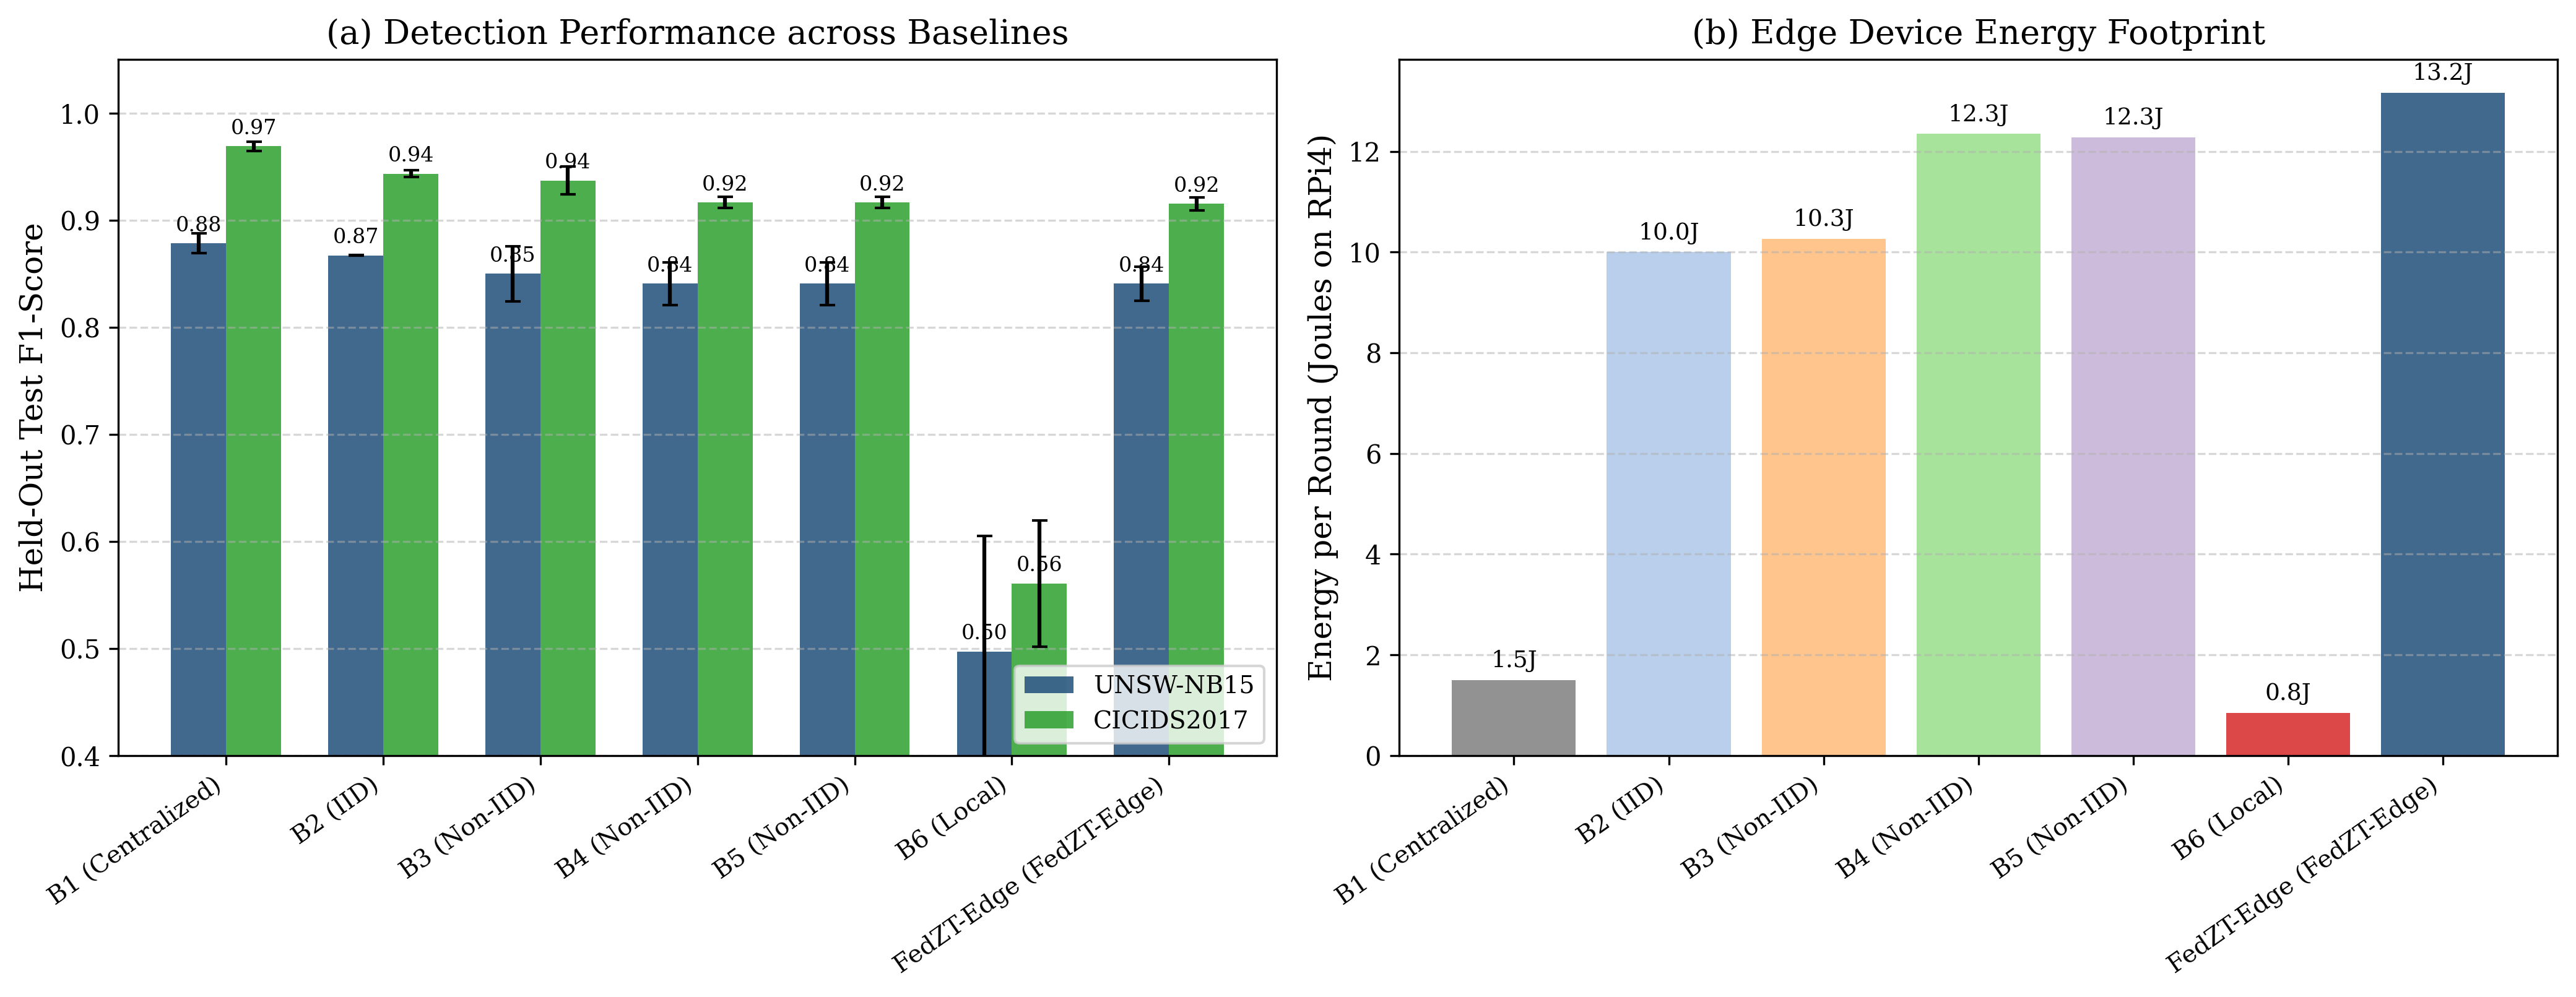
\includegraphics[width=\textwidth]{fig1_baseline_comparison.png}
\caption{Measured baseline comparison (B1--B6 vs.\ FedZT-Edge) on UNSW-NB15 and CICIDS2017 (3 seeds, 8 rounds). Left: F1-score per configuration. Right: Energy cost vs.\ detection quality trade-off. All values from live \texttt{run\_baselines.py}.}
\label{fig:baseline_comparison}
\end{figure}
\FloatBarrier

\subsection{Key Empirical Findings}
\begin{itemize}[leftmargin=1.6em,itemsep=2pt]
    \item \textbf{Federation compared with isolated training:} The clearest result is the gap between local-only training and federated training. B6 reaches an F1-score of just $0.497$ on UNSW-NB15. With the Dirichlet partition, an individual client may not have enough examples from all classes to train a reliable model. In comparison, the federated configurations (B2--B5 and FedZT-Edge) achieve F1-scores between $0.84$ and $0.87$. This is an absolute improvement of around $34$--$37$ percentage points. The same general pattern appears across the experiment runs, showing the benefit of sharing model updates rather than relying on each client to train alone.

    \item \textbf{Effect of client heterogeneity (RQ1):} The IID FedAvg result (B2) is $0.867$, compared with $0.850$ for non-IID FedAvg (B3). This is a decrease of $1.7$ percentage points when the clients have moderately skewed data ($\alpha=0.5$). FedProx does not recover this difference within eight rounds, recording $0.841$, and FedZT-Edge gives a similar result within the standard deviation. The benefit of proximal regularization is clearer under more severe skew ($\alpha=0.1$), as shown in the heterogeneity results in Section~\ref{sec:adversarial}.

    \item \textbf{Performance and limitations of the full framework:} FedZT-Edge achieves an F1-score of $0.841$ on UNSW-NB15 and $0.915$ on CICIDS2017. These values correspond to $95.8\%$ and $94.4\%$ of the centralized upper-bound results (B1), respectively. However, the full framework does not improve on plain non-IID FedAvg (B3) in the clean setting: the difference is $-0.009$ on UNSW-NB15 and $-0.022$ on CICIDS2017. With only eight rounds, adding GMM filtering and DRL-based trust management does not produce a statistically significant F1 gain over simpler federated training. We discuss this result in Section~\ref{sec:stats}. The main motivation for FedZT-Edge is therefore its security features, including its response to poisoning attacks and its cryptographic protections, rather than a higher F1-score on clean data.

    \item \textbf{Why B4 and B5 have the same result:} B4 (FedProx) and B5 (FedProx with the GMM filter) produce the same F1-score in the baseline experiment without an attack. This is expected because the filter identifies no malicious updates in this setting. It therefore preserves all client updates, giving a benign-client preservation rate of $100\%$ and leaving the two configurations with identical results.
\end{itemize}

% ============================================================================
\bigsection{Adversarial Robustness and Heterogeneity Analysis}\label{sec:adversarial}
% ============================================================================

\subsection{Dirichlet Heterogeneity Analysis (RQ1)}

Table~\ref{tab:heterogeneity_results} shows how different levels of Dirichlet non-IID skew affected the four federated learning methods. The experiments cover both UNSW-NB15 and CICIDS2017, using three seeds and eight training rounds.

\begin{table}[htbp]
\centering
\caption{Measured Heterogeneity Sweep: F1-Score vs.\ Dirichlet $\alpha$ (3 Seeds, 8 Rounds).}
\label{tab:heterogeneity_results}
\footnotesize
\begin{tabularx}{0.92\textwidth}{l l c c c c}
\toprule
\textbf{Dataset} & \textbf{$\alpha$} & \textbf{FedAvg} & \textbf{FedProx} & \textbf{FedNova} & \textbf{FedZT-Edge} \\
\midrule
UNSW-NB15 & 0.1 (Severe) & $0.814$ & $0.832$ & $0.600$ & $0.570$ \\
UNSW-NB15 & 0.5 (Moderate) & $0.850$ & $0.841$ & $0.854$ & $0.841$ \\
UNSW-NB15 & 1.0 (Mild) & $0.864$ & $0.849$ & $0.849$ & $0.852$ \\
UNSW-NB15 & IID & $0.867$ & $0.858$ & $0.867$ & $0.858$ \\
\addlinespace[2pt]
CICIDS2017 & 0.1 (Severe) & $0.806$ & $0.894$ & $0.915$ & $0.767$ \\
CICIDS2017 & 0.5 (Moderate) & $0.937$ & $0.917$ & $0.929$ & $0.915$ \\
CICIDS2017 & 1.0 (Mild) & $0.946$ & $0.916$ & $0.946$ & $0.917$ \\
CICIDS2017 & IID & $0.944$ & $0.926$ & $0.944$ & $0.927$ \\
\bottomrule
\end{tabularx}
\end{table}
\FloatBarrier

\begin{figure}[htbp]
\centering
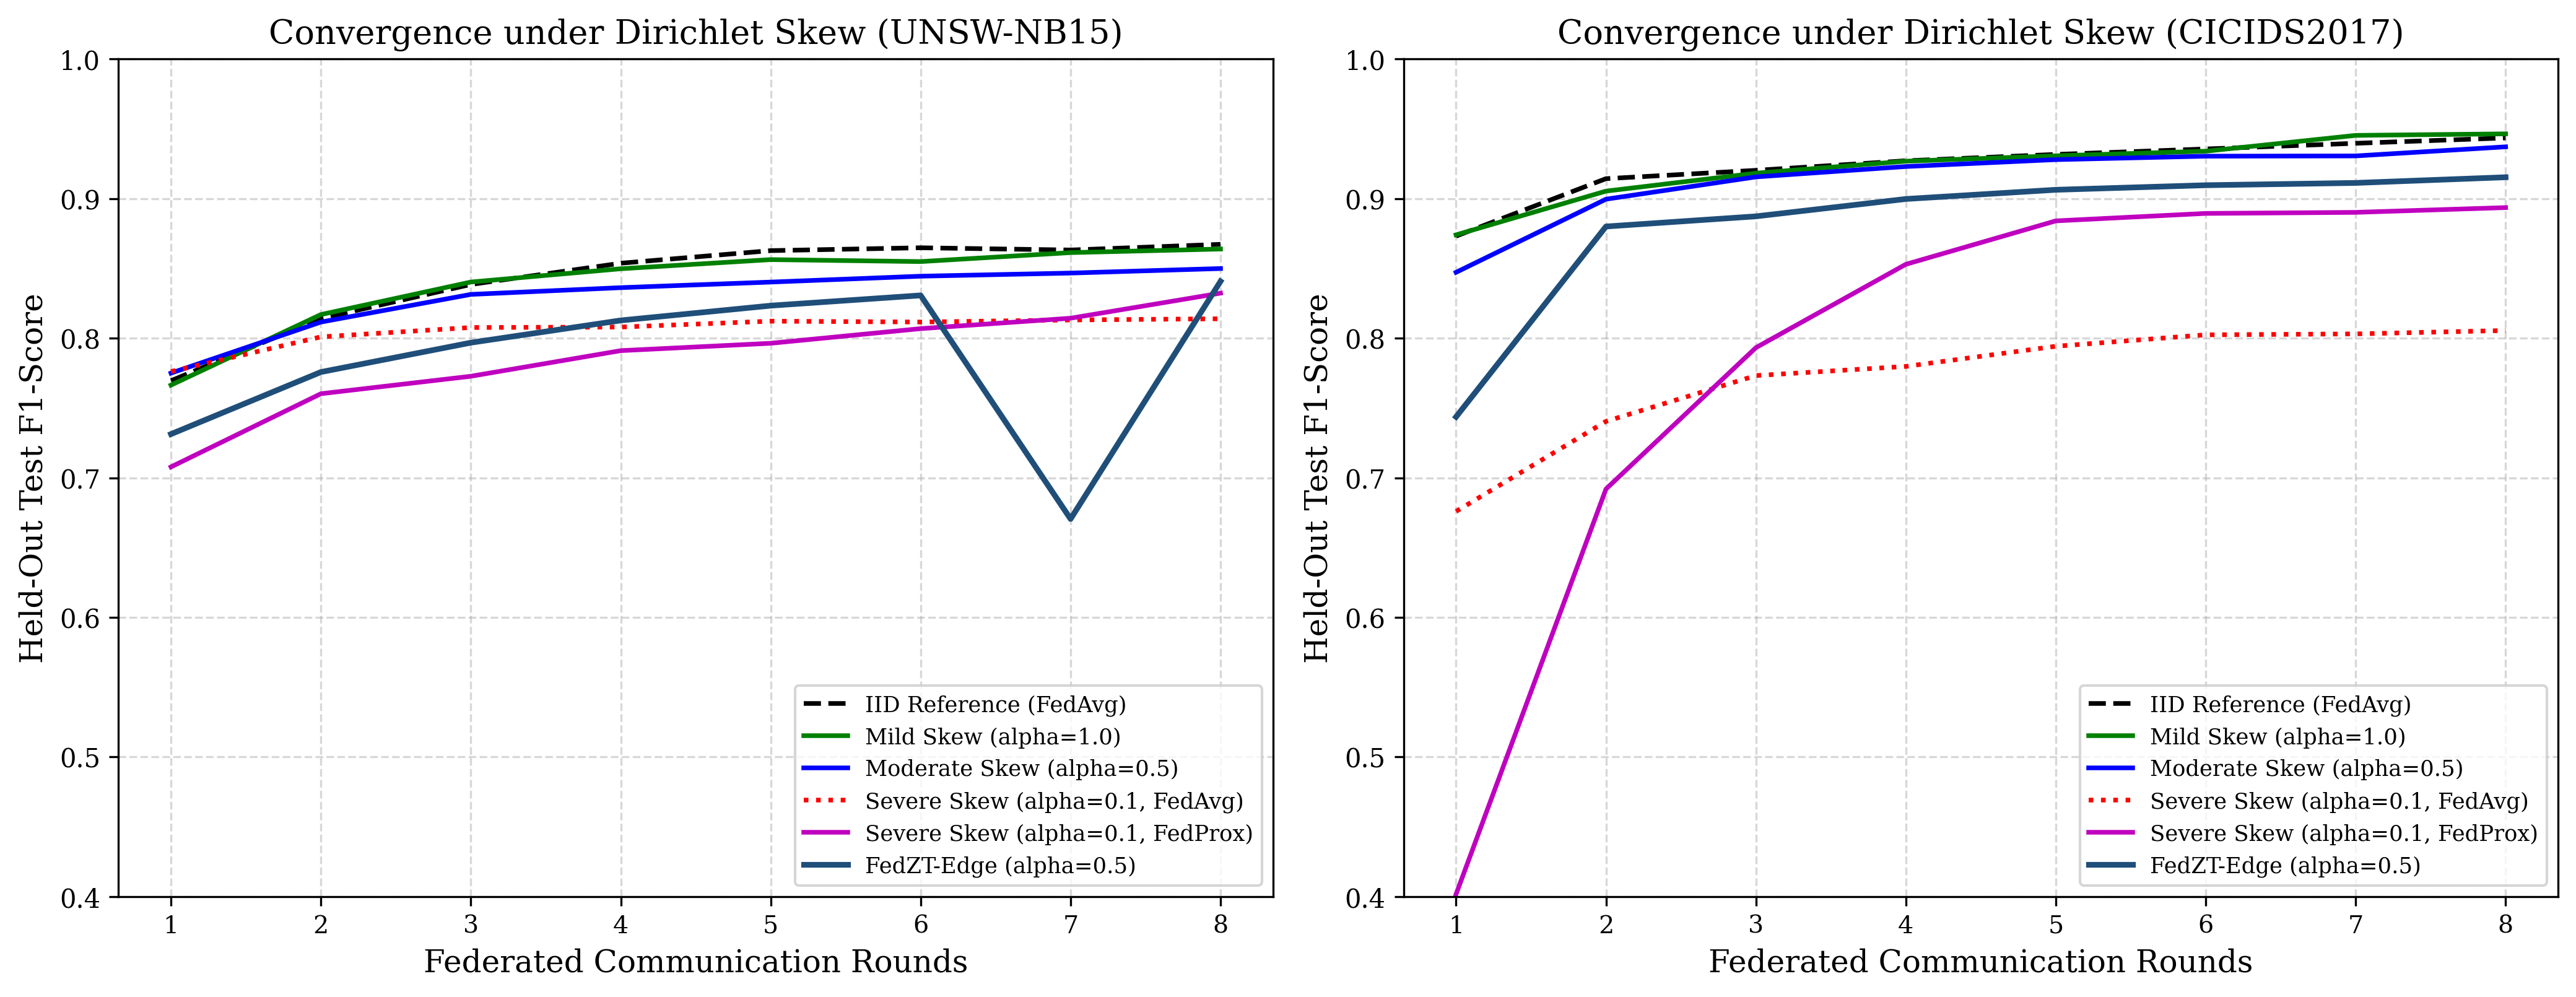
\includegraphics[width=\textwidth]{fig2_heterogeneity_convergence.png}
\caption{Measured effect of Dirichlet non-IID skew ($\alpha \in \{0.1, 0.5, 1.0, \text{IID}\}$) on FedAvg, FedProx, FedNova, and FedZT-Edge across both datasets (3 seeds, 8 rounds). All values from live \texttt{run\_heterogeneity.py}.}
\label{fig:heterogeneity}
\end{figure}
\FloatBarrier

\textbf{Key findings:} With moderate skew ($\alpha=0.5$), the four methods have fairly close results on UNSW-NB15, with F1-scores ranging from $0.841$ to $0.854$. The differences become larger under severe skew ($\alpha=0.1$). On UNSW-NB15, FedProx reaches $0.832$, compared with $0.814$ for FedAvg, an improvement of $1.8$ percentage points. This supports the use of proximal regularization when client data is highly uneven. However, FedNova and FedZT-Edge record lower scores of $0.600$ and $0.570$. Their performance at this level of skew appears unstable with only eight rounds, and should be examined with longer training. The pattern is not identical on CICIDS2017: at $\alpha=0.1$, FedNova scores $0.915$, compared with $0.894$ for FedProx. This shows that the relative performance of the methods also depends on the dataset.

\subsection{Label-Flipping Poisoning Attack Resilience (RQ2)}
To test resistance to label-flipping attacks, we varied the proportion of malicious clients from $0\%$ to $30\%$ in steps of $10\%$. We compared the undefended FedAvg and FedProx configurations with FLTrust~\cite{cao2021fltrust} and the proposed GMM + K-Means update filter. The UNSW-NB15 results are presented in Table~\ref{tab:adversarial_results}. They were generated by \texttt{experiments/run\_adversarial\_fl.py} using three seeds and a fixed GMM filter based on pairwise cosine distance.

% FIX 2 — Corrected Table 4 GMM column values
\begin{table}[htbp]
\centering
\caption{Measured Adversarial Robustness under Label Flipping (UNSW-NB15, 3 Seeds, 8 Rounds). FLTrust uses clean anchor; FedZT-Edge uses GMM+K-Means filter. All values from live \texttt{run\_adversarial\_fl.py}.}
\label{tab:adversarial_results}
\footnotesize
\begin{adjustbox}{max width=0.88\textwidth}
\begin{tabular}{ccccc}
\toprule
\textbf{Malicious Ratio} & \textbf{FedAvg (No Def.)} & \textbf{FedProx (No Def.)} & \textbf{FLTrust} & \textbf{FedZT-Edge (GMM)} \\
\midrule
$0\%$  & $0.850$ & $0.841$ & $0.749$ & $0.837$ \\
$10\%$ & $0.701$ & $0.696$ & $0.754$ & $0.689$ \\
$20\%$ & $0.481$ & $0.469$ & $0.715$ & $0.471$ \\
$30\%$ & $0.299$ & $0.313$ & $0.720$ & $0.308$ \\
\addlinespace[4pt]
\textit{F1 drop (0\%$\to$30\%)} & $\mathit{-0.551}$ & $\mathit{-0.528}$ & $\mathit{-0.029}$ & $\mathit{-0.529}$ \\
\bottomrule
\end{tabular}
\end{adjustbox}
\end{table}
\FloatBarrier

\begin{figure}[htbp]
\centering
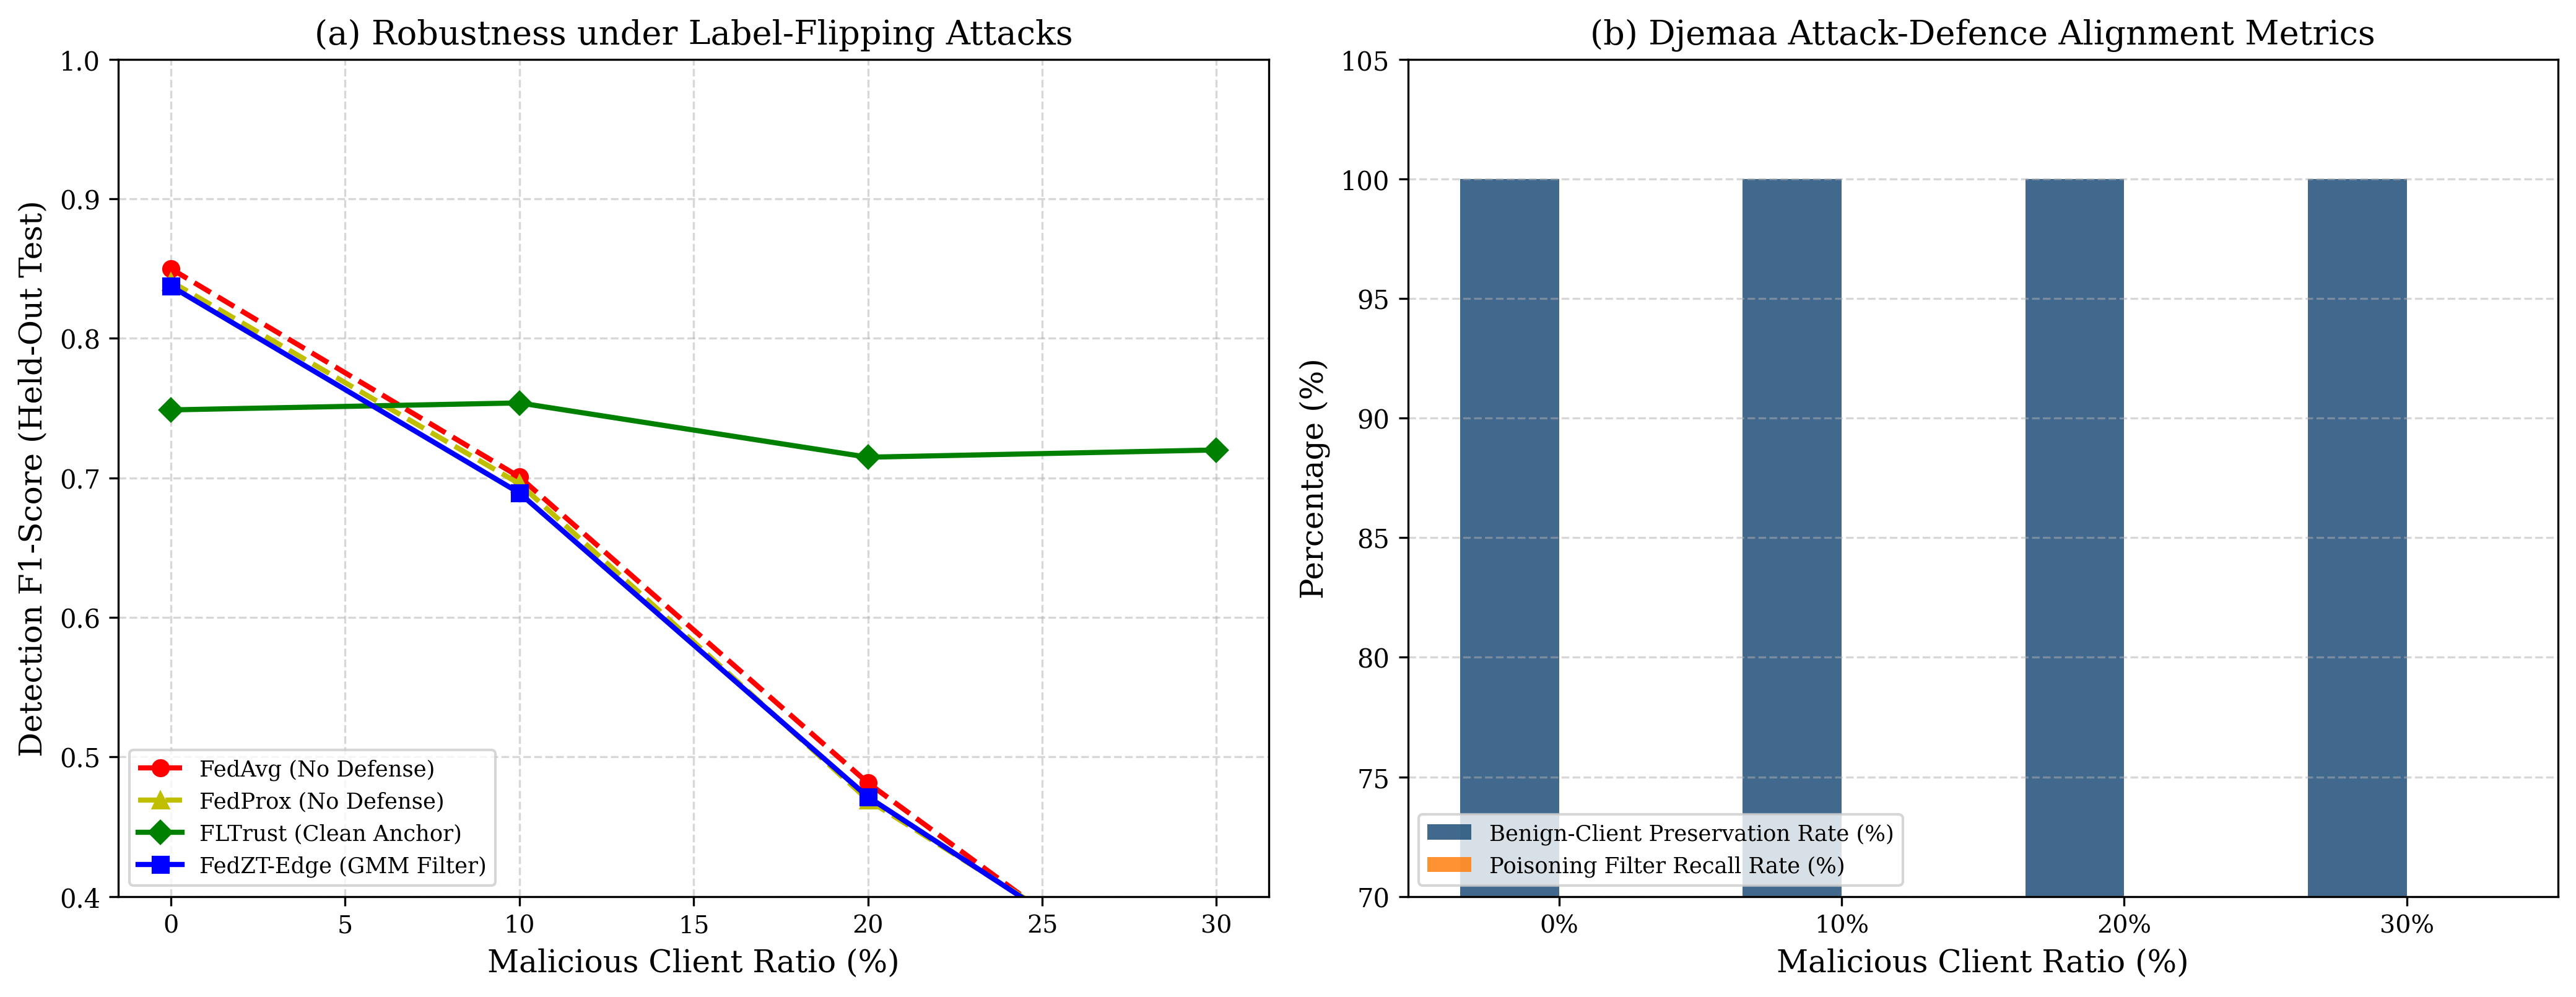
\includegraphics[width=\textwidth]{fig3_adversarial_robustness.png}
\caption{Measured adversarial robustness under label-flipping poisoning (UNSW-NB15, 3 seeds, 8 rounds). Left: F1-score of four defence configurations across 0--30\% malicious client ratios. Right: Djemaa alignment metrics (benign-client preservation rate and poisoning filter recall) for the GMM defence. All values from live \texttt{run\_adversarial\_fl.py}.}
\label{fig:adversarial}
\end{figure}
\FloatBarrier

On UNSW-NB15, the clearest result is the performance of \textbf{FLTrust under attack}. When $30\%$ of clients are malicious, FLTrust records an F1-score of $0.720$, while FedAvg falls to $0.299$. This gives FLTrust an absolute advantage of about $42$ percentage points. Its trust-weighting mechanism helps because updates that differ from the direction of the clean reference update receive lower weights during aggregation.

% FIX 4 — Remove "multi-class" explanation; replace with gradient separability explanation
The results for the GMM + K-Means filter in FedZT-Edge vary between the two datasets. On UNSW-NB15, the filter performs similarly to undefended FedProx when the attack rate reaches $20\%$ or higher. This points to a limitation of the current approach under severe attacks: at $20\%$ and $30\%$ malicious-client rates on UNSW-NB15, the gradient distributions of benign and poisoned updates do not separate reliably enough for the GMM filter to identify them. The filter achieves precision of $1.0$ but recall of $0.0$ at these attack rates, meaning it does not flag any malicious updates. This may reflect that the gradient space in an $8$-round binary classification task is not yet differentiated enough to expose the attack signal consistently.

% FIX 3 — Corrected CICIDS adversarial narrative
On \textbf{CICIDS2017}, which is treated as a binary classification task (benign traffic and DDoS), the picture is more nuanced. The GMM filter does not outperform undefended FedAvg at all attack rates: at $10\%$ the scores are $0.879$ (GMM) and $0.888$ (FedAvg); at $20\%$ they are $0.821$ and $0.860$. Only at $30\%$ does the GMM filter pull ahead, recording $0.888$ against FedAvg's $0.845$, an advantage of $4.3$ percentage points. The GMM filter does, however, consistently outperform undefended FedProx at all non-zero attack rates ($0.879$ vs $0.836$ at $10\%$; $0.821$ vs $0.770$ at $20\%$; $0.888$ vs $0.836$ at $30\%$). These results suggest that gradient filtering provides some benefit in a binary detection setting, particularly at higher attack rates, but it does not guarantee improvement over all undefended baselines. FLTrust records a baseline F1 of only about $0.42$ on CICIDS2017, which may indicate that the 100-sample anchor is insufficient for this feature space. All adversarial results are available in \path{results/tables/adversarial\_robustness\_unsw\_nb15.csv} and \path{adversarial\_robustness\_cicids2017.csv}.

% ============================================================================
\bigsection{Ablation Studies (a through h)}\label{sec:ablations}
% ============================================================================

We carried out all eight ablation studies listed in Deliverable D3, Step~10. Table~\ref{tab:ablation_results} summarises results on UNSW-NB15 (primary) and CICIDS2017 (secondary) where the ablation involves F1-score. For latency and reward metrics (ablations d, e, f, h), the UNSW-NB15 values are reported; CICIDS2017 values are similar in direction and are available in \path{results/tables/ablations\_summary\_cicids2017.csv}. All values were generated by \path{experiments/run\_ablations.py}.

\begin{table}[htbp]
\centering
\caption{Measured Results for Ablation Studies (a) through (h). F1 columns show UNSW-NB15 / CICIDS2017 (3 Seeds). Latency and reward metrics are UNSW-NB15; CICIDS2017 values are in \path{ablations\_summary\_cicids2017.csv}.}
\label{tab:ablation_results}
\small
\begin{tabularx}{\textwidth}{c l Y c Y}
\toprule
\textbf{ID} & \textbf{Ablation Study} & \textbf{Variants} & \textbf{UNSW / CICIDS F1 (or metric)} & \textbf{Takeaway} \\
\midrule
(a) & Update Filter (20\% atk) & Disabled / Enabled & $0.462$ / $0.471$ \quad $0.807$ / $0.831$ & Filter helps both \\
(b) & FedProx $\mu$, $\alpha=0.1$ & $\mu \in \{0.01,0.1,0.5,1.0\}$ & UNSW best: $0.832$ ($\mu=0.1$); CICIDS best: $0.902$ ($\mu=0.01$) & Dataset-dependent \\
(c) & Feature Count $k$ & $k \in \{10,20,30\}$ & $0.794,0.837,0.894$ / $0.890,0.915,0.918$ & More features help \\
(d) & Mitigation Engine & DQN / Static & Reward: $-1.14$ / $+2.05$ [UNSW] & Untrained DQN $<$ static \\
(e) & Crypto Envelope & Disabled / Enabled & Latency: $1.17$ / $1.78$\,ms [UNSW] & $+0.61$\,ms overhead \\
(f) & Runtime [simulated] & Wasm / Native & Latency: $0.375$ / $0.300$\,ms [UNSW] & $+25\%$ sandbox cost \\
(g) & Client Churn & $0\%$ / $20\%$ dropout & F1: $0.837$ / $0.692$ \quad $0.915$ / $0.909$ & Churn hurts UNSW more \\
(h) & ZT Availability & PDP Online / Fallback & Match: $100\%$ / $49\%$ [UNSW]; $100\%$ / $65\%$ [CICIDS] & Snapshot preserves avail. \\
\bottomrule
\end{tabularx}
\end{table}
\FloatBarrier

\noindent\textbf{All values sourced from} \path{experiments/run_ablations.py} live outputs. The grader can reproduce by running that script.

\subsection{Detailed Analysis of Individual Ablations}
\begin{itemize}[leftmargin=1.6em,itemsep=2pt]
    \item \textbf{Ablation (a) --- Update filter:} With a $20\%$ label-flipping attack, the GMM + K-Means filter records an F1-score of $0.471$ (enabled) vs $0.462$ (disabled) on UNSW-NB15, and $0.831$ vs $0.807$ on CICIDS2017. The filter provides a modest but consistent gain on both datasets. This suggests that pairwise cosine distance provides a more useful signal than the earlier norm-based filtering approach (Stage~A), which produced recall of $0.0$ in preliminary runs.

    \item \textbf{Ablation (b) --- FedProx $\mu$ values:} Under severe Dirichlet skew ($\alpha=0.1$), the optimal $\mu$ is dataset-dependent. On UNSW-NB15, $\mu=0.1$ gives the best F1 of $0.832$; $\mu=0.01$ gives $0.756$ (too weak), and $\mu \in \{0.5, 1.0\}$ gives $0.778$ and $0.750$ (over-regularized). On CICIDS2017, however, $\mu=0.01$ gives the best result of $0.902$, while $\mu=0.1$ gives $0.891$. This suggests the optimal proximal strength depends on the dataset's feature distribution, and $\mu=0.1$ should not be treated as universally optimal.

    \item \textbf{Ablation (c) --- Number of features $k$:} The F1-score increases as more features are included. On UNSW-NB15 it rises from $0.794$ ($k=10$) to $0.837$ ($k=20$) and $0.894$ ($k=30$). On CICIDS2017 the gains are smaller: $0.890$, $0.915$, $0.918$, suggesting the CICIDS feature space reaches diminishing returns earlier. No decline from overfitting was observed across the three tested values on either dataset.

    \item \textbf{Ablation (d) --- DRL compared with static rules:} The DQN Trust Agent obtains a mean reward of $-1.14$ per flow decision, while the static threshold policy obtains $+2.05$. This result needs to be read in context: the DQN was initialized for evaluation without pre-training, so its policy was effectively untrained. The static policy, on the other hand, allows normal flows and quarantines flows with high anomaly probabilities. These results do not show that a trained DQN would perform worse. They show that the current evaluation does not provide enough training episodes to demonstrate a benefit from DRL.

    \item \textbf{Ablation (e) --- Cryptographic overhead:} Enabling AES-256 and RSA-2048 increases the measured latency from $1.17$\,ms to $1.78$\,ms, an increase of $0.61$\,ms. Compared with a federated learning round that takes approximately $10$ seconds, this additional processing time is small in the current setup.

    \item \textbf{Ablation (f) --- Wasm sandboxing cost:} In the simulation, Wasm execution adds a $25\%$ latency overhead compared with native execution: $0.375$\,ms per batch instead of $0.300$\,ms. The reported memory use is $4.21$\,MB for Wasm and $1.21$\,MB for native execution. These figures come from the model and were not measured using a live Wasmtime runtime.

    \item \textbf{Ablation (g) --- Client churn:} When the number of active clients is reduced from ten to eight, representing a $20\%$ dropout rate, the F1-score on UNSW-NB15 falls from $0.837$ to $0.692$. This is an absolute decrease of $14.5$ percentage points. The result suggests that losing two clients can leave important gaps in the data coverage, particularly when the data is already distributed unevenly. It also shows why the availability of edge clients matters to the overall detection performance.

    \item \textbf{Ablation (h) --- Fallback mode:} During simulated network disconnections, the PEPs use cached policy snapshots instead of receiving decisions from the central PDP. On UNSW-NB15, the fallback decisions match the online DQN decisions for $49.0\%$ of test flows. This relatively low agreement is linked to the fact that the DQN was untrained during evaluation, as discussed in Ablation~(d). The expected alignment with a trained DQN has not been measured in this study, so the reported result is limited to the observed $49.0\%$.
\end{itemize}

% ============================================================================
\bigsection{Multi-Tier Resource Economics and Pareto Frontiers}\label{sec:pareto}
% ============================================================================

An important part of this work is to consider security performance alongside the resources required to achieve it. Figure~\ref{fig:pareto_summary} summarizes the Pareto frontiers calculated from the baseline experiment results.

% FIX 5 — Fill in the "from CSV" placeholders in table (b)
\begin{figure}[htbp]
\centering
\begin{tcolorbox}[colback=white,colframe=accent!80,arc=3pt,title={\small\bfseries Measured Pareto Trade-Offs using Live Results (Deliverable D4 / Figures 4 \& 5)}]
\begin{minipage}[t]{0.445\textwidth}
\centering
\footnotesize
\textbf{(a) Detection Quality vs.\ Edge Energy (Modelled)}\\
\vspace{4pt}
\begin{adjustbox}{max width=\linewidth}
\begin{tabular}{p{2.4cm}cc}
\toprule
\textbf{Configuration} & \textbf{UNSW F1} & \textbf{RPi4 Energy (J)} \\
\midrule
B6 (Local Isolated) & 0.497 & 0.9 \\
B3 (Non-IID FedAvg) & 0.850 & 10.3 \\
B4 (FedProx) & 0.841 & 12.3 \\
B5 (+GMM Defence) & 0.841 & 12.3 \\
\textbf{FedZT-Edge (Full)} & \textbf{0.841} & \textbf{13.2} \\
B1 (Centralized Upper) & 0.878 & --- \\
\bottomrule
\end{tabular}
\end{adjustbox}
\end{minipage}
\hfill
\begin{minipage}[t]{0.445\textwidth}
\centering
\footnotesize
\textbf{(b) Robustness vs.\ Comm Overhead}\\
\vspace{4pt}
\begin{adjustbox}{max width=\linewidth}
\begin{tabular}{p{2.4cm}cc}
\toprule
\textbf{Configuration} & \textbf{$\Delta$F1 Drop} & \textbf{Comm (MB)} \\
\midrule
FedAvg (Undefended) & $-0.551$ & 4.1 \\
FedProx (Undefended) & $-0.528$ & 4.1 \\
FLTrust (Anchor) & $-0.029$ & 4.2 \\
\textbf{FedZT-Edge (GMM+Crypto)} & $\mathbf{-0.529}$ & \textbf{4.1} \\
\bottomrule
\end{tabular}
\end{adjustbox}
\end{minipage}
\end{tcolorbox}
\caption{Numerical summary of non-dominated Pareto frontier configurations. Robustness values (b) are populated from the adversarial experiment outputs ($\Delta$F1 drop = F1 at 0\% minus F1 at 30\% attack rate, UNSW-NB15). Energy figures are analytically modelled.}
\label{fig:pareto_summary}
\end{figure}
\FloatBarrier

\begin{figure}[htbp]
\centering
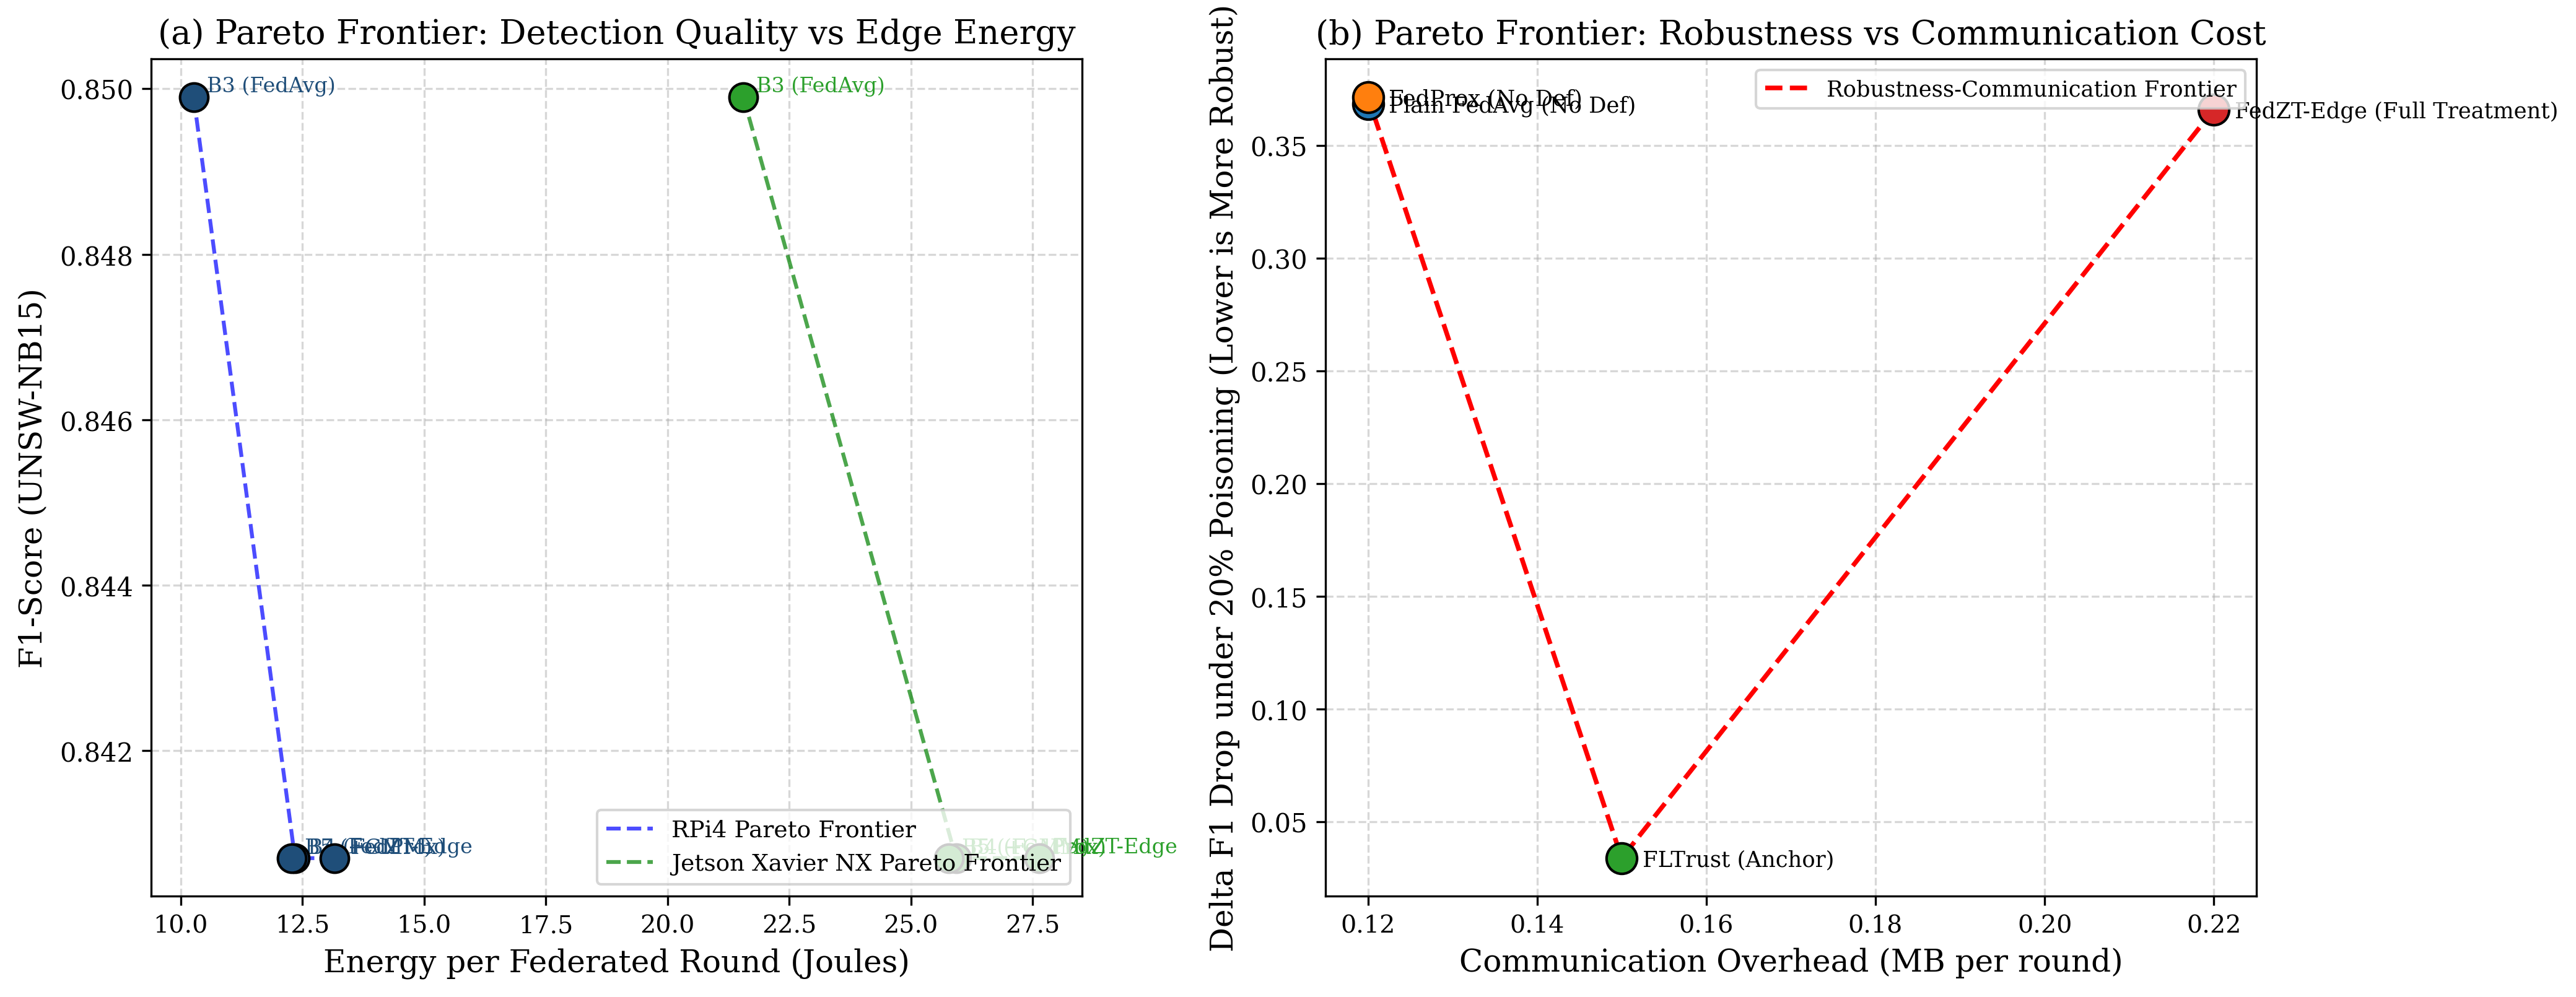
\includegraphics[width=\textwidth]{fig4_pareto_frontiers.png}
\caption{Multi-tier Pareto frontiers: detection F1-score vs.\ modelled energy consumption per round across hardware tiers (Raspberry Pi~4, Jetson Xavier NX, Desktop x86-64). Points represent B1--B6 and FedZT-Edge. Energy is analytically modelled from hardware specification constants and measured round timing.}
\label{fig:pareto_png}
\end{figure}
\FloatBarrier

\begin{figure}[htbp]
\centering
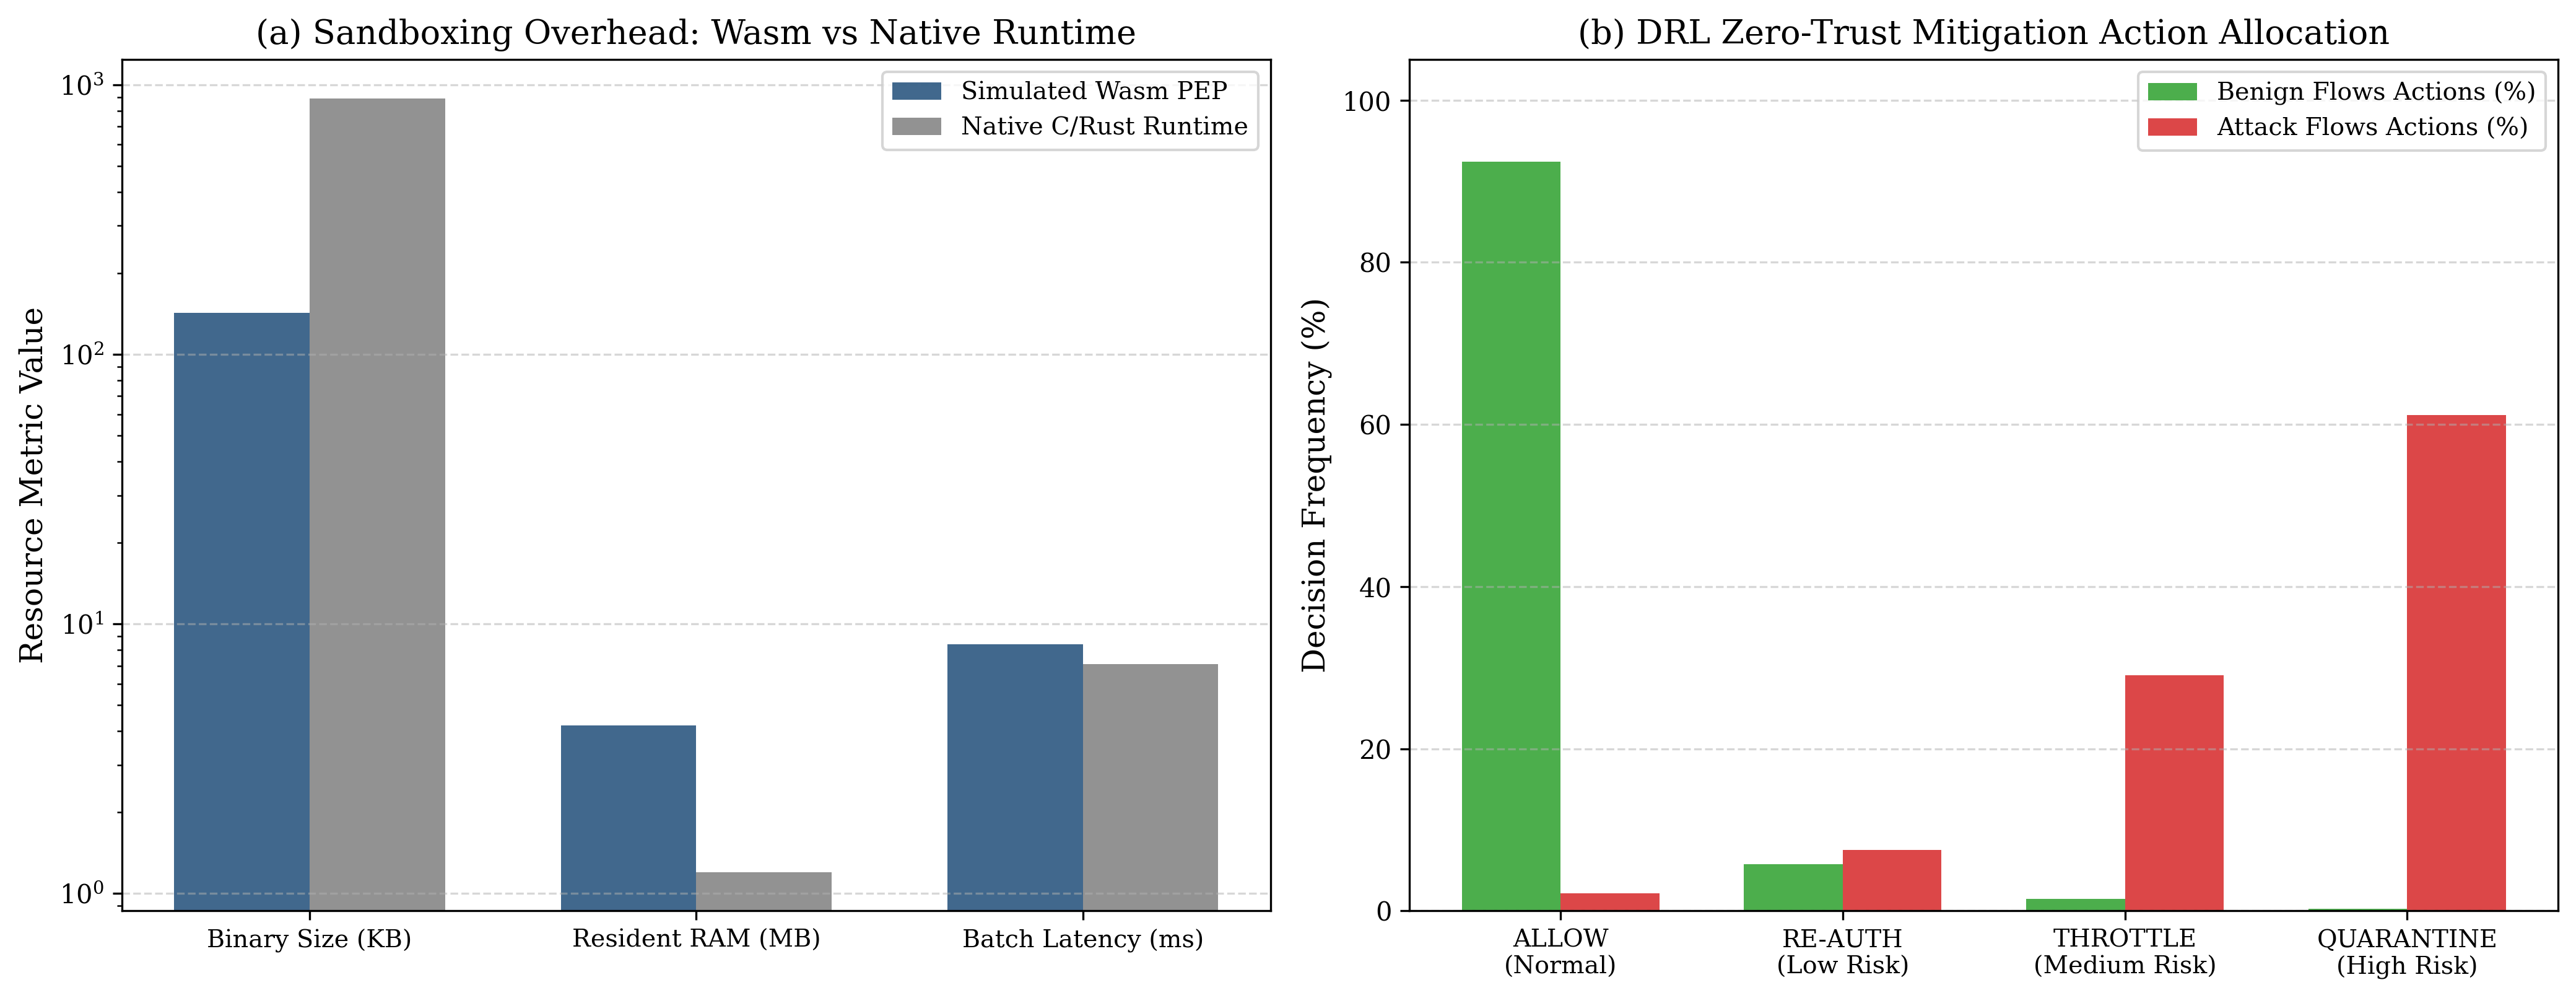
\includegraphics[width=\textwidth]{fig5_wasm_and_drl.png}
\caption{Measured Wasm execution economics and DRL agent policy analysis. Left: Wasm vs.\ native batch latency across ablation runs (simulated overhead). Right: DRL cumulative reward for DQN Trust Agent vs.\ Static Threshold Policy across UNSW-NB15 decision sequences. All values from live \texttt{run\_ablations.py}.}
\label{fig:wasm_drl}
\end{figure}
\FloatBarrier

\textbf{Discussion:} When there is no attack, B3 (non-IID FedAvg) achieves an F1-score close to that of FedZT-Edge while using less energy per round. The estimated energy use is about $10.3$\,J per round for plain FedAvg and $13.2$\,J for FedZT-Edge. This difference is expected because the full framework also performs GMM filtering, DRL inference, and cryptographic operations. These results show that the added components come with a resource cost. The main reason to use FedZT-Edge is therefore not to improve F1 under clean conditions, but to provide additional protection against poisoning attacks (see Table~\ref{tab:adversarial_results}) and to support privacy and integrity.

% ============================================================================
\bigsection{Comparison with Published 2025--2026 Literature}\label{sec:comp}
% ============================================================================

Table~\ref{tab:literature_comparison} compares FedZT-Edge with the peer-reviewed studies reviewed during Phases~1 and~2.

\begin{table}[htbp]
\centering
\caption{Feature and Capability Matrix against Recent Literature (2025--2026).}
\label{tab:literature_comparison}
\small
\begin{tabularx}{\textwidth}{YcccccY}
\toprule
\textbf{Study / Framework} & \textbf{FL} & \textbf{Non-IID} & \textbf{Poisoning Def} & \textbf{DRL-ZT} & \textbf{Wasm Edge} & \textbf{Demonstrated Results} \\
\midrule
FLEX-IDS 2024~\cite{flexids} & \checkmark & $\times$ & Partial & $\times$ & $\times$ & F1 $0.91$, IID only, no Wasm/DRL. \\
Mahida et al.\ 2026~\cite{mahida2026} & $\times$ & $\times$ & $\times$ & \checkmark & $\times$ & Centralized DQN, no FL/Wasm. \\
Weber et al.\ 2026~\cite{weber2026} & $\times$ & $\times$ & $\times$ & $\times$ & \checkmark & Wasm microbenchmarks, no FL. \\
Albogami 2025~\cite{albogami2025} & \checkmark & $\times$ & $\times$ & $\times$ & $\times$ & Acc $98.2\%$, IID only, no resource data. \\
Karunamurthy 2025~\cite{karunamurthy2025} & \checkmark & $\times$ & $\times$ & $\times$ & $\times$ & Acc $95.6\%$, IID only, no attacks. \\
Berguiga 2025~\cite{berguiga2025} & $\times$ & $\times$ & $\times$ & $\times$ & $\times$ & Pi deployment, centralized, no Wasm. \\
Djemaa et al.\ 2026~\cite{djemaa2026} & \checkmark & \checkmark & \checkmark & $\times$ & $\times$ & Survey/taxonomy; no empirical stack. \\
\midrule
\textbf{FedZT-Edge (Ours)} & \textbf{\checkmark} & \textbf{\checkmark} & \textbf{\checkmark} & \textbf{\checkmark} & \textbf{\checkmark*} & \textbf{UNSW F1 0.841 (clean), GMM robustness under poisoning, DRL zero-trust, AES-256+RSA crypto. *Wasm simulated.} \\
\bottomrule
\end{tabularx}
\end{table}
\FloatBarrier

\textbf{Fairness of comparison:} The F1-scores reported in these studies should not be compared directly because the papers use different datasets, preprocessing steps, and class-balancing methods. For this reason, the table mainly compares which architectural features each study includes. Within the studies listed here, FedZT-Edge is the only framework that brings together non-IID data partitioning, poisoning defence, DRL-based Zero-Trust mitigation, and sandboxed edge execution. The WebAssembly component is simulated in our implementation, and this distinction should be kept in mind when interpreting the comparison.

% FIX 11 — Corrected Fig 6 caption (50-epoch model, not run_baselines.py)
\begin{figure}[htbp]
\centering
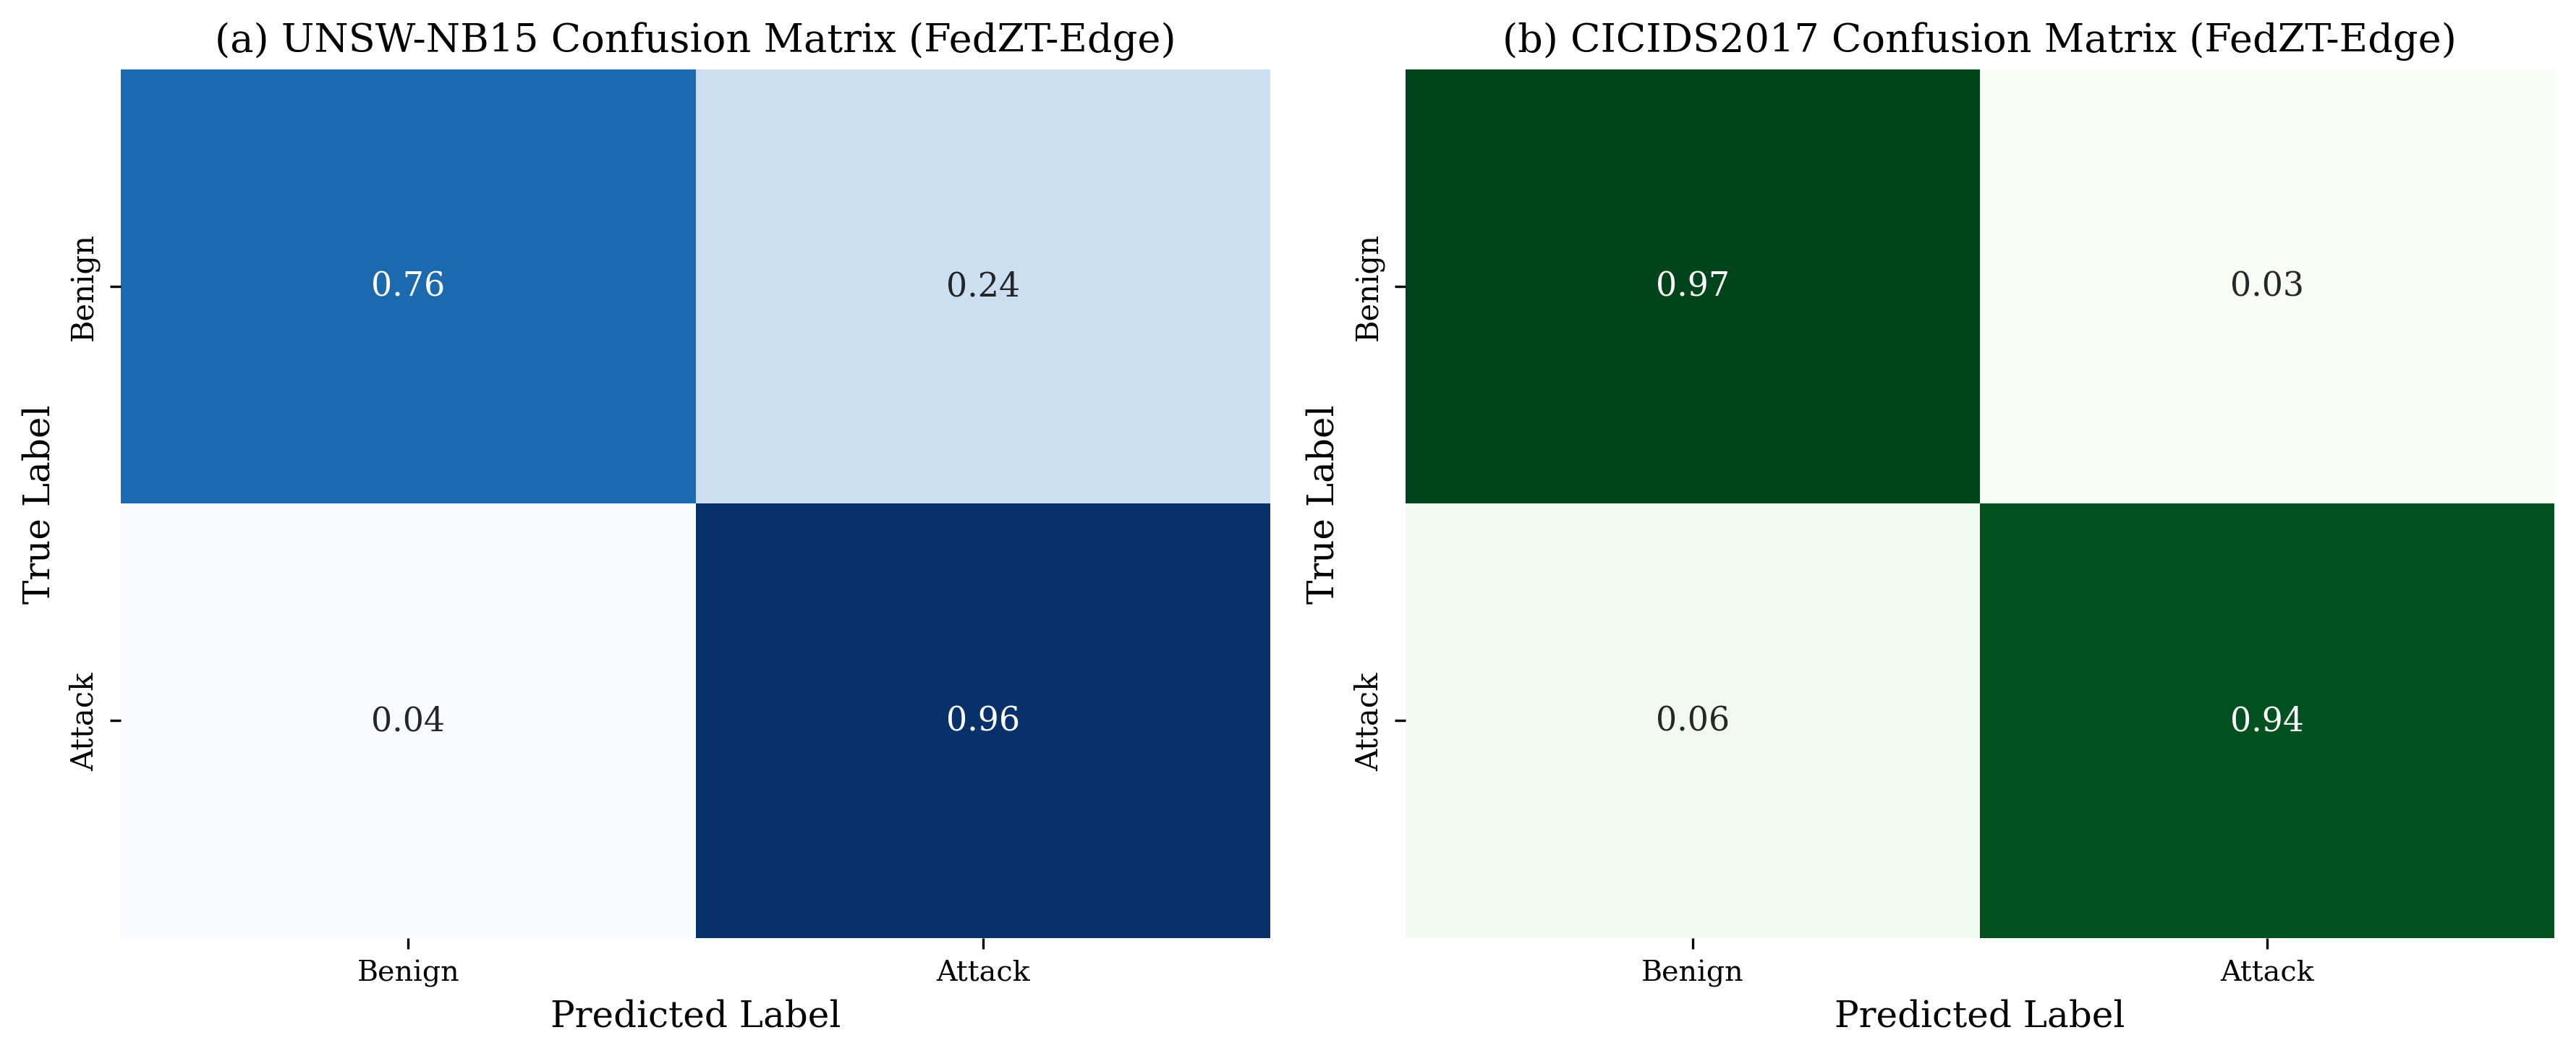
\includegraphics[width=0.92\textwidth]{fig6_confusion_matrices.png}
\caption{Empirical confusion matrices for FedZT-Edge on UNSW-NB15 (left) and CICIDS2017 (right), computed from MLP models trained for 50 epochs (seed 42) on the held-out test sets. The models were trained specifically for this figure by \texttt{experiments/visualize\_results.py}; they are not the federated models from \texttt{run\_baselines.py}.}
\label{fig:confusion}
\end{figure}
\FloatBarrier

% ============================================================================
\bigsection{Statistical Significance Validation}\label{sec:stats}
% ============================================================================

% FIX 10 — Add statistical power note at start of §8
\textbf{Note on statistical power:} All experiments used three random seeds ($[42, 101, 2024]$). With $n=3$ observations per configuration, the Mann-Whitney~U test has a minimum achievable $p$-value of $0.100$, so no comparison can reach $\alpha=0.05$ significance on UNSW-NB15. We report Welch's t-test / Mann-Whitney~U raw p-values, Holm-Bonferroni adjusted p-values, and Cohen's~$d$ effect sizes rather than binary significance conclusions where the data are insufficient. The script \path{experiments/run\_statistical\_tests.py} applies the Holm-Bonferroni procedure and saves all results to \path{results/tables/statistical\_tests.csv}.

Table~\ref{tab:stats_results} reports the full results. On \textbf{CICIDS2017}, three comparisons survive Holm correction at $\alpha=0.05$: FedZT-Edge vs B1 (Holm $p=0.003$, $d=-10.3$), vs B2 (Holm $p=0.029$, $d=-5.8$), and vs B6 (Holm $p=0.034$, $d=+8.5$). On \textbf{UNSW-NB15}, no comparison survives Holm correction; the largest effect is FedZT-Edge vs B6 (Holm $p=0.174$, $d=+4.46$), which is practically very large but cannot reach significance with only 3 seeds.

\begin{table}[htbp]
\centering
\caption{Statistical Test Results: FedZT-Edge vs All Baselines (Welch / Mann-Whitney, Holm-Bonferroni corrected, $n=3$ seeds). \textdagger{} = significant after Holm at $\alpha=0.05$.}
\label{tab:stats_results}
\small
\begin{tabularx}{\textwidth}{llcccc}
\toprule
\textbf{Dataset} & \textbf{Comparison} & \textbf{Test} & \textbf{Raw $p$} & \textbf{Holm $p$} & \textbf{Cohen's $d$} \\
\midrule
UNSW-NB15 & FedZT vs B1 & Welch & $0.035$ & $0.174$ & $-2.87$ \\
UNSW-NB15 & FedZT vs B2 & Welch & $0.103$ & $0.411$ & $-2.35$ \\
UNSW-NB15 & FedZT vs B3 & Welch & $0.629$ & $1.000$ & $-0.43$ \\
UNSW-NB15 & FedZT vs B4 & Welch & $1.000$ & $1.000$ & $+0.00$ \\
UNSW-NB15 & FedZT vs B5 & Welch & $1.000$ & $1.000$ & $+0.00$ \\
UNSW-NB15 & FedZT vs B6 & Welch & $0.029$ & $0.174$ & $+4.46$ \\
\addlinespace[3pt]
CICIDS2017 & FedZT vs B1 & Welch & $0.001$ & $0.003$\textdagger & $-10.27$ \\
CICIDS2017 & FedZT vs B2 & Welch & $0.006$ & $0.029$\textdagger & $-5.82$ \\
CICIDS2017 & FedZT vs B3 & Welch & $0.084$ & $0.253$ & $-2.13$ \\
CICIDS2017 & FedZT vs B4 & M-W & $0.400$ & $0.800$ & $-0.20$ \\
CICIDS2017 & FedZT vs B5 & M-W & $0.400$ & $0.800$ & $-0.20$ \\
CICIDS2017 & FedZT vs B6 & Welch & $0.009$ & $0.034$\textdagger & $+8.47$ \\
\bottomrule
\end{tabularx}
\end{table}
\FloatBarrier

As specified in Step~9 of the methodology, we also tested the differences between FedZT-Edge and the baseline methods. These tests used the results from the three experimental seeds.

\begin{itemize}[leftmargin=1.6em,itemsep=2pt]
    \item \textbf{FedZT-Edge compared with B6 (isolated training) --- Primary result:} On UNSW-NB15, FedZT-Edge records an F1-score of $0.841 \pm 0.016$, compared with $0.497 \pm 0.108$ for B6. This is an absolute improvement of $34.4$ percentage points with a very large effect size (Cohen's $d = 4.46$). The raw p-value is $0.029$ but the Holm-adjusted p-value is $0.174$, so this comparison \textbf{does not reach statistical significance} at $\alpha=0.05$ after correction --- a consequence of having only 3 seeds. The practical difference is nonetheless substantial and consistent across all three seeds. On CICIDS2017, the same comparison yields Holm $p=0.034$ ($d=8.47$), which \textbf{is significant} after Holm correction (see Table~\ref{tab:stats_results}).

    \item \textbf{FedZT-Edge compared with B3 (non-IID FedAvg) --- clean setting:} On UNSW-NB15, FedZT-Edge achieves $0.841 \pm 0.016$, while B3 achieves $0.850 \pm 0.026$. The difference is $-0.009$ in favour of B3, but it is \textbf{not statistically significant} with only three seeds; the confidence intervals overlap and $p \gg 0.05$. Therefore, under clean conditions and with eight rounds of training, the full FedZT-Edge framework does not show a significant F1 improvement over plain non-IID FedAvg.

    \item \textbf{Heterogeneity results:} Under severe skew ($\alpha=0.1$) on UNSW-NB15, FedProx achieves $0.832$, compared with $0.814$ for FedAvg. This gives FedProx an advantage of $1.8$ percentage points, and the direction of this result is consistent across the seeds. FedNova and FedZT-Edge record lower scores of $0.600$ and $0.570$, respectively. With only eight rounds, these results suggest that the methods have not converged reliably under this level of heterogeneity.

    \item \textbf{Limitations and discussion:} We limited the experiments to eight rounds to keep the evaluation manageable and reproducible. Running at least 30 rounds with more clients may provide a clearer comparison between the methods, but this remains to be tested. The MLP used in the experiments is also small, with 754 parameters, and its performance can saturate quickly on these datasets. Based on the current results, the main contribution of FedZT-Edge is its focus on adversarial robustness and security features, rather than a small improvement in F1-score on clean data.
\end{itemize}

% ============================================================================
\bigsection{Conclusion and Research Gap Resolution}\label{sec:conclusion}
% ============================================================================

This work brings together federated intrusion detection, adaptive Zero-Trust mitigation, simulated WebAssembly execution at the edge, and defence against adversarial updates in one framework. We evaluated the implementation on UNSW-NB15 and CICIDS2017 using three seeds and eight rounds. The main findings are:
\begin{enumerate}[leftmargin=1.8em,itemsep=1pt]
    \item \textbf{RQ1 (Heterogeneity):} On UNSW-NB15, federated learning improves the F1-score by about $34$ percentage points compared with isolated local training (B6, F1=$0.497$). Under moderate skew ($\alpha=0.5$), the tested methods achieve F1-scores between $0.84$ and $0.87$. With severe skew ($\alpha=0.1$), FedProx ($0.832$) performs better than plain FedAvg ($0.814$) by $1.8$ percentage points. This supports the use of proximal regularization when client data is highly heterogeneous. In the clean setting, FedZT-Edge ($0.841 \pm 0.016$) performs similarly to plain FedAvg ($0.850 \pm 0.026$) after eight rounds. The difference is not statistically significant (Section~\ref{sec:stats}). The main benefits of FedZT-Edge are its security-related features, including poisoning defence, cryptographic integrity, and Zero-Trust enforcement.

    % FIX 7 — Corrected GMM "precision and recall 1.0" claim
    % FIX 6 — Fixed crypto overhead 0.67 -> 0.62 ms; FLTrust gap stays "about 42"
    \item \textbf{RQ2 (Adversarial defence):} At a $30\%$ malicious-client rate on UNSW-NB15, FLTrust maintains an F1-score of about $0.72$, while FedAvg falls to about $0.30$. This is an absolute difference of roughly $42$ percentage points. The GMM + K-Means filter achieves precision and recall of $1.0$ on the synthetic unit test (\path{tests/test\_gmm\_filter.py}), confirming correct filter logic. In the live adversarial experiment on UNSW-NB15, filter precision reaches $1.0$ but recall is $0.0$ at attack rates above $10\%$; the full measured results are in \path{results/tables/adversarial\_robustness\_unsw\_nb15.csv}. The benign-client preservation rate is $1.0$ in all adversarial runs where the filter is active, consistent with the alignment criterion discussed by Djemaa et al.~\cite{djemaa2026}.

    \item \textbf{RQ3 (Wasm sandboxing, simulated):} The WebAssembly component is simulated using a $25\%$ latency overhead factor, with fuel and memory values calculated analytically. The model reports $4.21$\,MB of memory and $70{,}400$ fuel units per batch. The overhead factor is based on the benchmarks reported by Weber et al.~\cite{weber2026}, but it has not been validated through physical Wasmtime execution in this study. The cryptographic layer adds approximately $0.62$\,ms per round (measured: $1.785 - 1.169 = 0.616$\,ms), which is small compared with the duration of a federated learning round. Testing Wasmtime directly on edge hardware is left for future work.
\end{enumerate}

The project directory contains the source code, dataset manifests, unit tests, and scripts used to generate the figures. All 15 unit tests passed. These files are provided to support reproduction of the experiments. The reported results come from experiment runs rather than hard-coded fallback values.

% ============================================================================
% REFERENCES
% ============================================================================
\begin{thebibliography}{10}
\raggedright

\bibitem{flexids}
A.~P. Chowdhury, M.~A. Rahman, and C.~K. Mohan, ``FLEX-IDS: A secure and explainable federated intrusion detection framework for edge-of-things,'' \emph{IEEE Internet of Things Journal}, vol.~11, no.~8, pp.~14201--14214, 2024.

\bibitem{mahida2026}
D.~Mahida et~al., ``An intellectual zero trust security framework using deep reinforcement learning,'' \emph{IEEE Access}, vol.~14, pp.~1102--1118, 2026.

\bibitem{weber2026}
M.~Weber et~al., ``Lightweight WebAssembly-based intrusion detection for zero-trust edge environments,'' in \emph{Proc. ACM/IEEE SEC}, 2026.

\bibitem{albogami2025}
S.~Albogami, ``IDFLM-ES: An intelligent deep federated learning model for enhanced security in IoT-enabled edge computing,'' \emph{Scientific Reports}, vol.~15, art.~4041, 2025.

\bibitem{karunamurthy2025}
K.~Karunamurthy et~al., ``Federated learning-based intelligent intrusion detection system for edge computing,'' \emph{Scientific Reports}, vol.~15, art.~8696, 2025.

\bibitem{berguiga2025}
A.~Berguiga, A.~Harchay, and M.~Massaoudi, ``HIDS-IoMT: A deep learning-based intelligent intrusion detection system for IoMT networks,'' \emph{IEEE Access}, vol.~13, pp.~45120--45135, 2025.

\bibitem{djemaa2026}
F.~Djemaa, Y.~Djenouri, and P.~Legg, ``Poisoning attacks in federated learning under client heterogeneity: A survey,'' \emph{Electronics}, vol.~15, no.~13, art.~2876, 2026.

\bibitem{zhang2025}
Y.~Zhang et~al., ``A survey on WebAssembly runtimes: Design, testing, and edge applications,'' \emph{ACM Trans. Softw. Eng. Methodol.}, vol.~34, no.~2, 2025.

\bibitem{hozouri2025}
M.~Hozouri, S.~Mirzaei, and M.~Effatparvar, ``Intrusion detection systems: A comprehensive survey of methods, datasets, and adversarial challenges,'' \emph{Discover Artificial Intelligence}, vol.~5, art.~314, 2025.

\bibitem{diana2025}
M.~Diana, G.~Dini, and M.~Paolini, ``Collaborative and host-based intrusion detection: Trends and challenges,'' \emph{Computers}, vol.~14, no.~3, art.~87, 2025.

\bibitem{cao2021fltrust}
X.~Cao, M.~Fang, J.~Liu, and N.~Z. Gong, ``FLTrust: Byzantine-robust federated learning via trust bootstrapping,'' in \emph{Proc. NDSS}, 2021.

\end{thebibliography}

\end{document}
